\fontsize{13pt}{22.5pt}\selectfont

% ═══════════════════════════════════════════════════════════════
\section{XÂY DỰNG ỨNG DỤNG TRÌNH DIỄN TƯƠNG TÁC}
\label{ch:app}

\indent Các chương trước đã trình bày quá trình huấn luyện và so sánh năm thuật toán
học tăng cường trên ba môi trường game ba chiều. Tuy nhiên, kết quả huấn luyện dưới
dạng biểu đồ và bảng số liệu chưa phản ánh trực tiếp chất lượng hành vi của
tác nhân trong game. Để khép kín quy trình từ huấn luyện đến triển khai, đề tài xây
dựng thêm một ứng dụng trình diễn tương tác, cho phép người dùng lựa chọn môi trường,
lựa chọn chế độ chơi và lựa chọn mô hình đã huấn luyện cho tác nhân ngay trong game,
đồng thời tra cứu lại chính các số liệu huấn luyện đã phân tích ở
Chương~\ref{ch:results} mà không cần rời khỏi ứng dụng. Ứng dụng này vừa là công cụ
minh họa trực quan cho các kết quả so sánh, vừa chứng minh tính khả thi của việc triển
khai các mô hình ONNX đã huấn luyện vào một sản phẩm game hoàn chỉnh.

% ───────────────────────────────────────────────
\subsection{Mục tiêu và yêu cầu chức năng}
\label{sub:app-goal}

\indent Ứng dụng trình diễn được thiết kế với bốn nhóm yêu cầu chức năng chính. Nhóm
yêu cầu về lựa chọn nội dung chơi quy định ứng dụng phải cung cấp một màn
hình menu cho phép người dùng chọn một trong ba môi trường (Cross The Road, Capture
The Flag và Football Table) và một trong ba chế độ chơi tương ứng với các cách phân vai
giữa người chơi và tác nhân máy.

\indent Nhóm yêu cầu về các chế độ chơi quy định ba cách phân vai. Chế độ \textit{Người chơi} cho
phép người dùng trực tiếp điều khiển tác nhân bằng bàn phím, qua đó tự mình trải
nghiệm độ khó của nhiệm vụ mà tác nhân phải học. Chế độ \textit{Agent tự chơi} để
mô hình đã huấn luyện điều khiển toàn bộ tác nhân, phục vụ việc quan sát và đánh giá
trực quan chất lượng chính sách. Chế độ \textit{Chơi với Agent} kết hợp cả hai: người
chơi và tác nhân máy cùng xuất hiện trong một phiên chơi, với vai trò đồng đội hoặc
đối thủ tùy theo bản chất của từng môi trường.

\indent Nhóm yêu cầu về lựa chọn mô hình quy định rằng ở mọi chế độ có sự tham gia
của tác nhân máy, người dùng phải chọn được mô hình cụ thể (tương ứng với thuật toán
PPO, SAC, MA-POCA, MAPPO, DQN hoặc các phiên bản huấn luyện khác nhau) cho tác nhân sử
dụng. Yêu cầu này biến ứng dụng thành một công cụ so sánh trực quan: người dùng có thể
lần lượt chạy cùng một môi trường với các mô hình khác nhau để quan sát sự khác biệt
về hành vi, hoặc cho hai mô hình đối đầu trực tiếp trong môi trường Football Table.

\indent Nhóm yêu cầu cuối cùng là tra cứu kết quả huấn luyện ngay trong ứng dụng. Thay vì
buộc người xem mở TensorBoard hoặc lật lại báo cáo, menu được bổ sung hai tab chuyên
biệt: một tab hiển thị đường cong phần thưởng và bảng thống kê của cả năm thuật toán
trên môi trường đang chọn, một tab tổng hợp và xếp hạng các thuật toán trên cả ba môi
trường. Hai tab này phải phủ đúng phạm vi thực nghiệm của Chương~\ref{ch:results}:
mười lăm lần chạy, không thiếu thuật toán nào. Nhờ đó, người dùng có thể xem số liệu
trước rồi chuyển sang tab chơi để đối chiếu với hành vi quan sát được.

\indent Bên cạnh các yêu cầu chức năng, ứng dụng còn phải thỏa mãn một ràng buộc quan
trọng về mặt kỹ thuật: không được phá vỡ cấu hình huấn luyện hiện có của các scene.
Ba scene môi trường vẫn được sử dụng hằng ngày cho việc huấn luyện, do đó mọi thay
đổi phục vụ chế độ chơi chỉ được phép diễn ra tại thời gian chạy khi người dùng đi
vào từ menu, còn khi mở scene trực tiếp trong Unity Editor để huấn luyện thì mọi
thứ phải giữ nguyên như cũ.

% ───────────────────────────────────────────────
\subsection{Kiến trúc hệ thống}
\label{sub:app-arch}

\indent Toàn bộ mã nguồn của ứng dụng trình diễn được tổ chức trong một thư mục riêng
\texttt{Assets/GameHub}, tách biệt hoàn toàn với mã nguồn của ba môi trường - vốn nằm
trong một gói riêng (Mục~\ref{sub:app-package}) và được ứng dụng tiêu thụ qua ranh giới
assembly. Hệ thống gồm các thành phần chính được tóm tắt trong
Bảng~\ref{tab:app_modules}.

% Bảng dài mười hai dòng mô tả nên không thể nằm gọn trong một trang. Dùng longtable
% thay cho table[H] để bảng tự ngắt sang trang sau và lặp lại dòng tiêu đề, thay vì bị
% tràn khỏi đáy trang như khi bị ghim cứng bằng [H].
\begingroup
\renewcommand{\arraystretch}{1.35}
\tablefont
\begin{longtable}{|p{4.4cm}|>{\raggedright\arraybackslash}p{9.1cm}|}
\caption{Các thành phần chính của ứng dụng trình diễn}
\label{tab:app_modules} \\
\hline
\textbf{Thành phần} & \textbf{Vai trò} \\
\hline
\endfirsthead
\hline
\textbf{Thành phần} & \textbf{Vai trò} \\
\hline
\endhead
\endfoot
\texttt{GameModeSelection} & Lớp tĩnh lưu lựa chọn của người dùng (môi trường, chế độ
chơi, tên mô hình); tồn tại xuyên suốt giữa các scene và quyết định scene nào
được nạp cho lựa chọn hiện tại. \\
\hline
\texttt{ModelRegistry} & Liệt kê và nạp các mô hình ONNX từ thư mục
\texttt{Resources/AgentModels} tại thời gian chạy. \\
\hline
\texttt{MainMenuUI} & Dựng toàn bộ giao diện menu ba tab bằng mã lệnh khi scene
\texttt{MainMenu} khởi động. \\
\hline
\texttt{UIBuilder} & Thư viện dựng thành phần giao diện (canvas, panel bo góc, nút,
văn bản) dùng chung cho menu và HUD. \\
\hline
\texttt{Preview3D} & Dựng bản sao ``chỉ có hình khối'' của prefab môi trường và render
bằng camera riêng ra \texttt{RenderTexture} để xem trước xoay được. \\
\hline
\texttt{TrainingDataStore} & Nạp tệp \texttt{training\_data.json} chứa đường cong và
thống kê huấn luyện thật đã xuất từ TensorBoard. \\
\hline
\texttt{UILineChart} & Biểu đồ đường tự vẽ bằng mesh trên uGUI, hiển thị nhiều chuỗi
reward trong cùng một hệ trục. \\
\hline
\texttt{GameModeApplier} & Lắng nghe sự kiện nạp scene; chọn số khu vực huấn luyện cần
giữ lại và cấu hình lại các tác nhân trong đó (loại hành vi, mô hình, chu kỳ quyết
định) theo lựa chọn từ menu. \\
\hline
\texttt{InGameHUD} & Giao diện phủ trong game: nút quay về menu, thông tin chế độ và
dòng hướng dẫn phím. \\
\hline
Các thành phần điều khiển & \texttt{CrossRoadHumanInput}, \texttt{PuzzleHumanInput},
\texttt{FootballHumanInput}: chuyển tín hiệu bàn phím thành hành động của tác nhân
ở chế độ người chơi. \\
\hline
\end{longtable}
\endgroup

\indent Luồng hoạt động của hệ thống được minh họa trong Hình~\ref{fig:app_flow}.
Khi người dùng bấm nút bắt đầu ở menu, các lựa chọn được ghi vào
\texttt{GameModeSelection} rồi scene môi trường tương ứng được nạp. Thành phần
\texttt{GameModeApplier} đăng ký với sự kiện \texttt{sceneLoaded} của Unity ngay từ
khi ứng dụng khởi động nhờ thuộc tính
\texttt{[Runtime\allowbreak Initialize\allowbreak On\allowbreak Load\allowbreak Method]},
nên nó luôn ở trạng thái sẵn sàng trước mọi lần chuyển scene; khi scene môi trường
được nạp xong, thành phần này kiểm tra xem người dùng có đi vào từ menu hay không. Nếu có, nó tìm các tác
nhân trong scene và cấu hình lại từng tác nhân theo chế độ đã chọn; nếu không (trường
hợp mở scene trực tiếp để huấn luyện), nó không can thiệp gì và scene giữ nguyên cấu
hình gốc. Cách tiếp cận dựa trên sự kiện này cho phép bổ sung đầy đủ chức năng chơi
game mà không cần sửa đổi bất kỳ scene môi trường nào.

\begin{figure}[H]
\centering
\begin{tikzpicture}[
    node distance=1.0cm and 2.0cm,
    box/.style={draw, rounded corners=2pt, align=center, minimum height=1.1cm,
                inner sep=5pt, font=\fontsize{11pt}{14pt}\selectfont},
    lbl/.style={font=\fontsize{10pt}{12pt}\selectfont, fill=white, inner sep=2pt},
    arr/.style={->, thick}
]
\node[box, fill=blue!10, text width=4.2cm] (menu) {Scene \texttt{MainMenu}\\ \texttt{MainMenuUI}};
\node[box, fill=orange!15, right=of menu, text width=5.6cm] (sel) {\texttt{GameModeSelection}\\ (môi trường, chế độ, mô hình)};
\node[box, fill=blue!10, below=of sel, text width=5.6cm] (scene) {Nạp scene môi trường\\ (CrossTheRoad / CaptureTheFlag\\ / Football)};
\node[box, fill=orange!15, below=of menu, text width=4.2cm] (applier) {\texttt{GameModeApplier}\\ (sự kiện \texttt{sceneLoaded})};
\node[box, fill=green!12, below=of applier, text width=4.6cm] (agent) {Cấu hình tác nhân\\ Heuristic / Inference\\ + mô hình ONNX};
\node[box, fill=green!12, below=of scene, text width=4.6cm] (hud) {\texttt{InGameHUD}\\ + điều khiển người chơi};

\draw[arr] (menu) -- node[lbl, above]{ghi lựa chọn} (sel);
\draw[arr] (sel) -- (scene);
\draw[arr] (scene) -- node[lbl, above]{thông báo} (applier);
\draw[arr] (applier) -- (agent);
\draw[arr] (applier) -- (hud);
\end{tikzpicture}
\caption{Luồng hoạt động của ứng dụng trình diễn}
\label{fig:app_flow}
\end{figure}

\indent Điểm mấu chốt trong khâu cấu hình tác nhân là việc chuyển đổi giữa các loại
hành vi của ML-Agents. Mỗi tác nhân đều mang một thành phần
\texttt{BehaviorParameters} quy định nguồn ra quyết định của nó: ở phe do người chơi
điều khiển, loại hành vi được đặt thành \texttt{HeuristicOnly} để hành
động lấy từ hàm \texttt{Heuristic}; ở chế độ tác nhân máy, loại hành vi được đặt thành
\texttt{InferenceOnly} và mô hình ONNX được nạp vào để mạng nơ-ron suy luận trực tiếp
trong engine. Nhờ hạ tầng suy luận tích hợp sẵn của Unity, quá trình suy luận diễn ra
cục bộ trên máy người chơi với chi phí tính toán không đáng kể, không cần bất kỳ tiến
trình Python nào như khi huấn luyện.

% ───────────────────────────────────────────────
\subsection{Giao diện menu và luồng sử dụng}
\label{sub:app-menu}

{\sloppy
\indent Khi khởi động ứng dụng, người dùng được đưa vào màn hình menu chính. Toàn bộ
giao diện được dựng bằng mã lệnh (không dùng prefab giao diện) và được tổ chức thành
ba tab: \textit{CHƠI}, \textit{THÔNG SỐ} và \textit{SO SÁNH}. Tab \textit{CHƠI}
(Hình~\ref{fig:app_menu}) chia màn hình thành hai cột: cột trái là khung xem trước
môi trường ở dạng ba chiều kèm tên, khẩu hiệu phân loại bài toán và mô tả ngắn; cột
phải là lưới nút chọn chế độ chơi, khu vực chọn mô hình, khối mô tả và nút bắt
đầu. Khối mô tả thay đổi động theo tổ hợp môi trường - chế độ đang chọn, hiển thị tóm
tắt luật chơi cùng sơ đồ phím điều khiển tương ứng, giúp người dùng nắm được cách chơi
trước khi vào game.\par}

\begin{figure}[H]
\centering
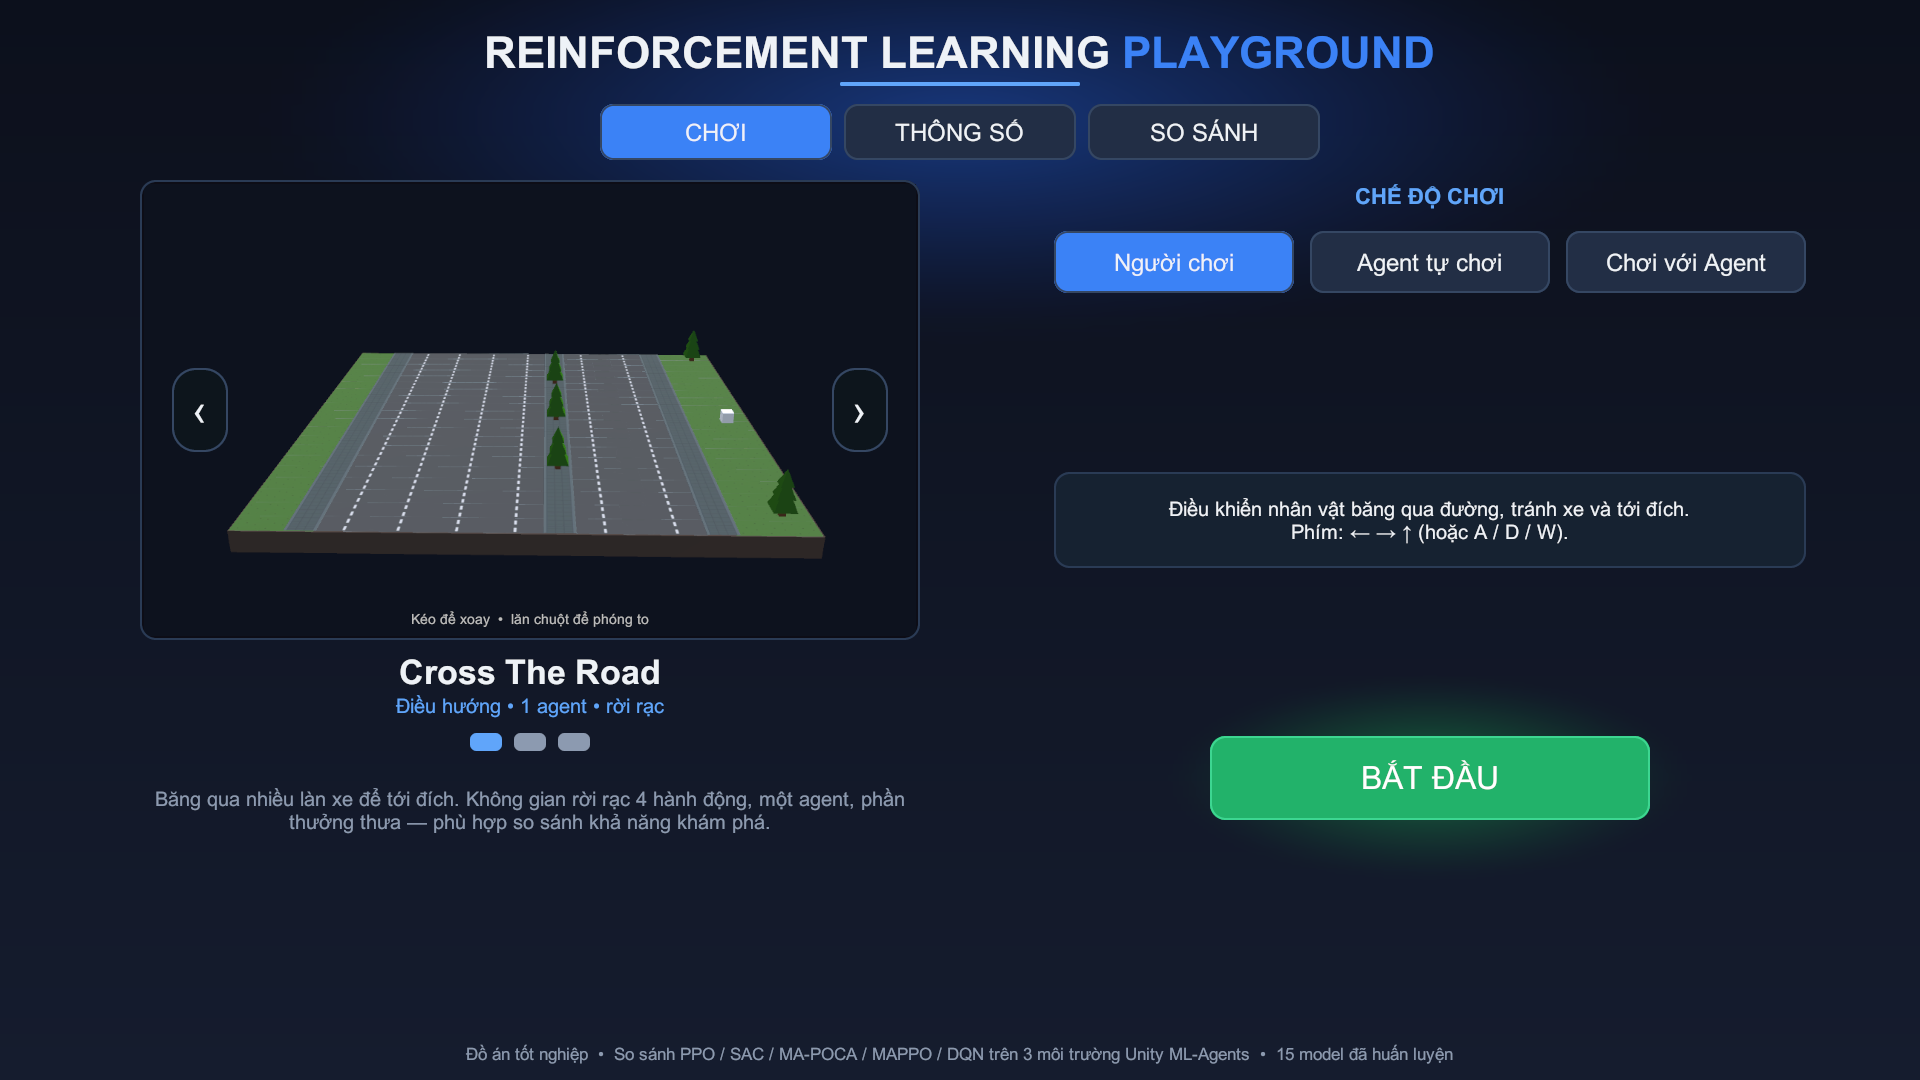
\includegraphics[width=0.85\textwidth]{image/app/app_menu_main.png}
\caption{Tab CHƠI của menu chính: khung xem trước ba chiều (trái) và các lựa
chọn chế độ chơi (phải)}
\label{fig:app_menu}
\end{figure}

{\sloppy
\indent Khung xem trước ba chiều do thành phần \texttt{Preview3D} đảm nhiệm. Thay vì
dùng ảnh tĩnh, thành phần này nạp prefab của môi trường từ thư mục
\texttt{Resources/\allowbreak EnvPrefabs} và sao chép chỉ các cặp lưới - vật liệu
(\texttt{MeshFilter} và \texttt{MeshRenderer}) sang một ``sân khấu'' đặt xa khu vực
menu. Nhờ chỉ giữ lại phần hình học, bản xem trước không mang theo mã điều khiển hay
thành phần vật lý nào, do đó không có mô phỏng nào chạy ngầm và không gây ảnh hưởng
chéo tới scene menu. Một camera riêng render sân khấu này ra \texttt{RenderTexture}
rồi gắn vào giao diện, cho phép kéo chuột để xoay và lăn chuột để phóng to; khi không
có thao tác nào, mô hình tự xoay chậm. Khoảng cách camera ban đầu được tính từ hộp bao
của toàn bộ hình khối nên mọi môi trường đều vừa khung mà không cần chỉnh tay; hai nút
mũi tên hai bên khung cho phép chuyển nhanh giữa ba môi trường theo kiểu băng chuyền.\par}

\indent Khu vực chọn mô hình chỉ xuất hiện khi chế độ đang chọn có sự tham gia của
tác nhân máy. Số lượng ô chọn mô hình cũng thay đổi theo ngữ cảnh: các tổ hợp chỉ
cần một mô hình sẽ hiển thị một ô duy nhất, riêng môi trường Football Table ở chế độ
\textit{Agent tự chơi} hiển thị hai ô riêng biệt cho đội Xanh và đội Đỏ
(Hình~\ref{fig:app_menu_models}), cho phép hai mô hình khác nhau đối đầu trực tiếp.
Nhãn của mỗi ô cũng được sinh theo ngữ cảnh (``Model cho cả 2 agent'', ``Model đội
Xanh'', ``Model agent đồng đội''\dots) để người dùng biết chính xác mô hình mình chọn
sẽ điều khiển ai. Danh sách mô hình trong mỗi ô được liệt kê tự động từ thư mục tài
nguyên, vì vậy khi bổ sung một mô hình mới chỉ cần sao chép tệp ONNX vào đúng thư mục
mà không phải sửa bất kỳ dòng mã nào. Mỗi ô hiển thị tên thuật toán ghép với mã lần
chạy (chẳng hạn ``MA-POCA \textperiodcentered{} ctf\_poca\_v2'') và tô đúng màu quy ước
của thuật toán đó, nên khi lần lượt duyệt qua năm mô hình của một môi trường, người
dùng biết ngay mình đang xem chính sách của thuật toán nào mà không phải thuộc lòng
quy ước đặt tên các lần chạy.

\begin{figure}[H]
\centering
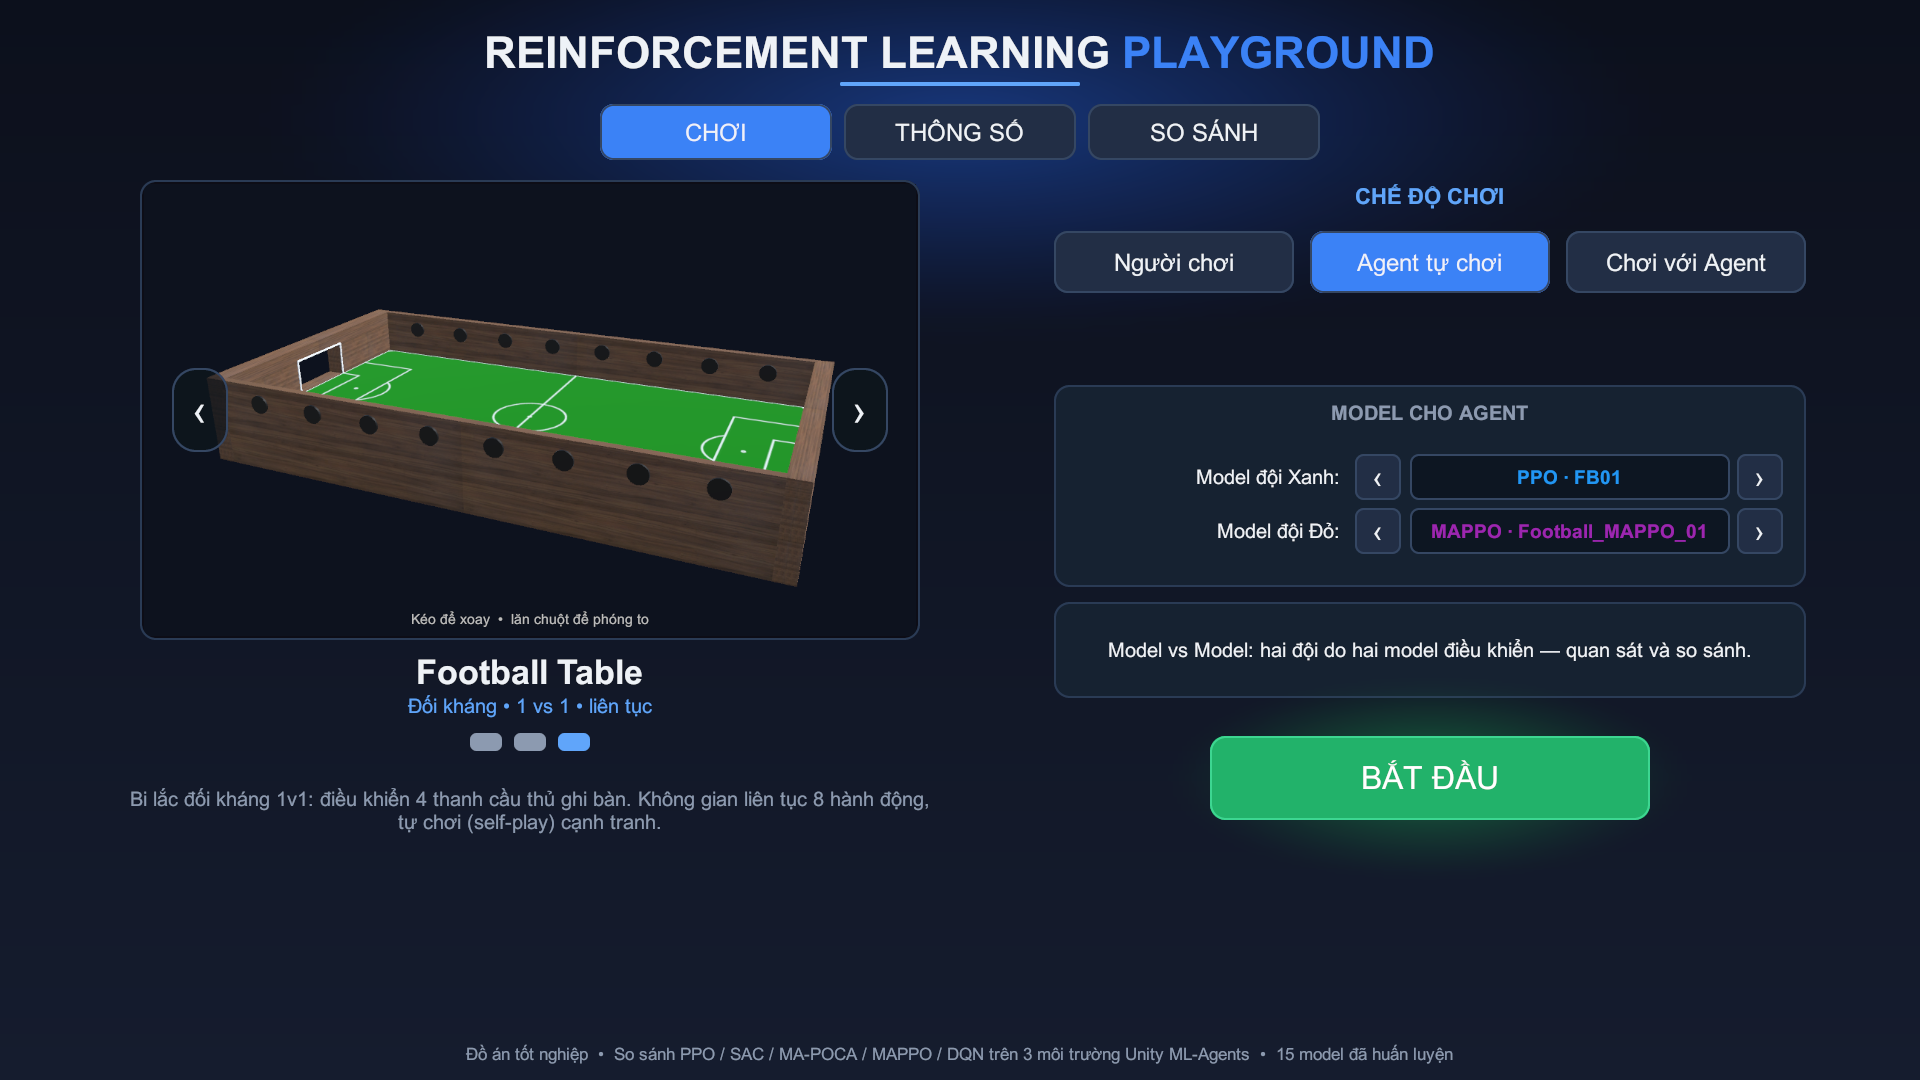
\includegraphics[width=0.85\textwidth]{image/app/app_menu_models.png}
\caption{Khu vực chọn mô hình khi Football Table ở chế độ Agent tự chơi:
hai ô chọn riêng cho đội Xanh và đội Đỏ}
\label{fig:app_menu_models}
\end{figure}

\indent Nút bắt đầu chỉ được kích hoạt khi mọi điều kiện đã đủ. Nếu thư mục mô hình
của môi trường đang chọn rỗng, hoặc nếu hai ô mô hình của Football Table được đặt vào
hai loại không gian hành động khác nhau, ứng dụng sẽ khóa nút bắt đầu và hiển thị một
dòng cảnh báo màu đỏ chỉ rõ nguyên nhân. Cách xử lý này giúp người dùng không
rơi vào tình huống bấm chơi rồi mới gặp lỗi giữa chừng.

\indent Trong mọi phiên chơi, một thanh thông tin mỏng được phủ ở mép trên màn hình,
hiển thị tên môi trường, chế độ chơi, mô hình đang sử dụng và nút quay về menu (hoặc
phím Esc); mép dưới màn hình là dòng nhắc phím điều khiển. Người dùng vì thế luôn
biết mình đang ở tổ hợp thực nghiệm nào và có thể quay lại menu để đổi lựa chọn bất
cứ lúc nào mà không phải khởi động lại ứng dụng.

% ───────────────────────────────────────────────
\subsection{Nạp mô hình ONNX tại thời gian chạy}
\label{sub:app-model}

\indent Mỗi lần huấn luyện trong Chương~\ref{ch:results} kết thúc, ML-Agents xuất
chính sách đã học ra một tệp ONNX. Để các tệp này dùng được trong ứng dụng, chúng
được sao chép vào cây thư mục tài nguyên của Unity theo quy ước mỗi môi trường một
thư mục con:

\begin{center}
\texttt{Assets/GameHub/Resources/AgentModels/\{CrossTheRoad | CaptureTheFlag |
Football\}/}
\end{center}

{\sloppy
\noindent Tên tệp được giữ đúng bằng mã của lần chạy huấn luyện (ví dụ
\texttt{ctr01}, \texttt{ctf\_mappo\_v2}), và tên này cũng chính là nhãn hiển thị trong
menu; nhờ vậy mô hình trong ứng dụng luôn truy vết được về đúng thư mục kết quả và
đúng biểu đồ đã phân tích ở Chương~\ref{ch:results}. Unity nhập mỗi tệp ONNX thành
một tài sản \texttt{ModelAsset} của gói suy luận tích hợp. Nhờ đó, ứng dụng liệt kê
được danh sách mô hình bằng lời gọi \texttt{Resources.LoadAll}, rồi gán mô hình đã
chọn cho tác nhân qua giao diện \texttt{SetModel} của ML-Agents, như minh họa trong
đoạn mã dưới đây.\par}

\begin{lstlisting}[language={[Sharp]C}, caption={Liệt kê và gán mô hình ONNX tại thời gian chạy}]
ModelAsset[] models =
    Resources.LoadAll<ModelAsset>("AgentModels/" + envName);

agent.SetModel(behaviorName, selectedModel);
behaviorParameters.BehaviorType = BehaviorType.InferenceOnly;
\end{lstlisting}

\indent Cách tổ chức này tách hoàn toàn dữ liệu mô hình khỏi mã nguồn: danh mục mô
hình trong menu phản ánh trực tiếp nội dung thư mục tài nguyên, nên việc bổ sung một mô
hình mới chỉ là thao tác sao chép tệp. Thao tác sao chép đó nay do chính kịch bản xuất
dữ liệu huấn luyện đảm nhiệm (Mục~\ref{sub:app-stats}): sau mỗi đợt huấn luyện, kịch bản
lấy tệp ONNX cuối cùng của từng lần chạy, đặt tên theo mã lần chạy rồi ghi vào đúng thư
mục con của môi trường. Nhờ vậy ứng dụng luôn đóng gói \textbf{toàn bộ mười lăm mô hình}
tương ứng với mười lăm lần chạy của Chương~\ref{ch:results}, liệt kê trong
Bảng~\ref{tab:app_models}; mỗi môi trường có đủ năm chính sách của năm thuật toán đặt
cạnh nhau, cho phép so sánh hành vi bằng mắt trên cùng một nhiệm vụ.

\begin{table}[H]
\centering
\caption{Mười lăm mô hình ONNX được đóng gói sẵn trong ứng dụng}
\label{tab:app_models}
\renewcommand{\arraystretch}{1.3}
\tablefont
\begin{tabular}{|p{3.0cm}|p{4.6cm}|p{3.8cm}|>{\centering\arraybackslash}p{1.6cm}|}
\hline
\textbf{Môi trường} & \textbf{Tệp mô hình} & \textbf{Thuật toán} & \textbf{Số bước} \\
\hline
\multirow{5}{*}{Cross The Road}
 & \texttt{ctr01} & PPO & 2,00M \\
\cline{2-4}
 & \texttt{CrossTheRoad\_SAC\_01} & SAC & 2,00M \\
\cline{2-4}
 & \texttt{ctr\_poca\_v1} & MA-POCA & 2,00M \\
\cline{2-4}
 & \texttt{ctr\_mappo\_v1} & MAPPO & 2,00M \\
\cline{2-4}
 & \texttt{ctr\_dqn\_v1} & DQN & 2,00M \\
\hline
\multirow{5}{*}{Capture The Flag}
 & \texttt{ctf\_ppo\_v1} & PPO & 1,70M \\
\cline{2-4}
 & \texttt{ctf\_sac\_v1} & SAC & 1,64M \\
\cline{2-4}
 & \texttt{ctf\_poca\_v2} & MA-POCA & 1,70M \\
\cline{2-4}
 & \texttt{ctf\_mappo\_v2} & MAPPO & 1,70M \\
\cline{2-4}
 & \texttt{ctf\_dqn\_v1} & DQN & 1,70M \\
\hline
\multirow{5}{*}{Football Table}
 & \texttt{FB01} & PPO (self-play) & 1,60M \\
\cline{2-4}
 & \texttt{Football\_SAC\_01} & SAC (self-play) & 1,60M \\
\cline{2-4}
 & \texttt{Football\_POCA\_01} & MA-POCA (self-play) & 1,60M \\
\cline{2-4}
 & \texttt{Football\_MAPPO\_01} & MAPPO (self-play) & 1,60M \\
\cline{2-4}
 & \texttt{football\_dqn\_v1} & DQN (rời rạc) & 1,60M \\
\hline
\end{tabular}
\end{table}

\indent Một chi tiết kỹ thuật phải xử lý riêng khi đóng gói đủ mười lăm mô hình là
\textit{không gian hành động}. Trên Cross The Road và Capture The Flag, cả năm thuật
toán đều dùng hành động rời rạc nên mọi tệp ONNX đều nạp được vào scene gốc. Riêng
Football Table, bốn thuật toán PPO, SAC, MA-POCA và MAPPO sinh chính sách hành động
liên tục tám kênh, còn DQN chỉ định nghĩa được trên hành động rời rạc nên lần chạy
\texttt{football\_dqn\_v1} dùng phiên bản tám nhánh ba mức của cùng bài toán
(Mục~\ref{sub:env-football}). Không gian hành động được khai báo trong thành phần
\texttt{BehaviorParameters} của scene và ML-Agents dựng bộ truyền động của tác nhân
ngay trong pha \texttt{OnEnable}, tức trước khi ứng dụng kịp can thiệp sau khi scene
nạp xong; vì thế không thể đổi kiểu hành động tại thời gian chạy như cách đổi mô hình.
Giải pháp là giữ song song hai bản scene Football: bản liên tục dùng cho bốn thuật toán
kia và bản rời rạc \texttt{FootballDiscrete} sinh tự động từ bản gốc bằng một kịch bản
trong trình soạn thảo. Khi người dùng chọn mô hình DQN, menu nạp bản rời rạc thay cho
bản gốc; phần còn lại của ứng dụng không thay đổi vì lớp tác nhân của Football vốn đã
chấp nhận cả hai kiểu hành động và tự quy đổi ba mức $\{0,1,2\}$ về $\{-1,0,+1\}$. Hệ
quả duy nhất người dùng nhìn thấy là ở chế độ \textit{Agent tự chơi} của Football Table,
hai ô chọn mô hình phải cùng loại hành động: menu khóa nút bắt đầu kèm dòng cảnh báo
nếu ghép DQN với một thuật toán liên tục, vì một trận đấu chỉ nạp được một scene.

% ───────────────────────────────────────────────
\subsection{Trực quan hóa kết quả huấn luyện trong ứng dụng}
\label{sub:app-stats}

\indent Một điểm khác biệt của ứng dụng so với một demo game thông thường là hai tab
số liệu được nhúng ngay trong menu. Số liệu hiển thị không phải là con số nhập tay mà
được trích xuất tự động từ chính các tệp nhật ký huấn luyện, nhờ vậy mọi lần huấn
luyện lại đều có thể cập nhật vào ứng dụng chỉ bằng một lệnh.

\subsubsection{Đường ống dữ liệu từ TensorBoard vào game}

\indent Trong quá trình huấn luyện, ML-Agents ghi các chỉ số ra tệp \texttt{tfevents}
trong thư mục \texttt{results/<run\_id>/}. Một kịch bản Python
(\texttt{export\_training\_data.py}) đọc các tệp này bằng \texttt{EventAccumulator}
của TensorBoard và thực hiện bốn bước xử lý nối tiếp. Kịch bản gộp chuỗi
\texttt{Environment/Cumulative Reward} của tất cả tệp nhật ký thuộc cùng một lần chạy
và sắp xếp theo số bước; làm mượt chuỗi bằng trung bình trượt để loại
bớt nhiễu giữa các tập; rút gọn chuỗi đã làm mượt xuống tối đa một trăm
hai mươi điểm cách đều nhằm giữ kích thước tệp nhỏ, phù hợp để nạp trong game; và cuối
cùng tính các thống kê tóm tắt gồm phần thưởng cuối, phần thưởng tốt nhất, trung
bình mười phần trăm cuối, bước hội tụ ước lượng và tổng số bước.

\indent Cùng lượt chạy đó, kịch bản còn làm hai việc nữa để dữ liệu và mô hình không
bao giờ lệch pha nhau. Thứ nhất, nó sao chép tệp ONNX cuối cùng của từng lần chạy vào
thư mục tài nguyên của ứng dụng dưới đúng tên mã lần chạy, bỏ qua tệp đã trùng kích
thước để Unity không phải nhập lại. Thứ hai, nó xác định không gian hành động của từng
mô hình bằng cách đọc thẳng tên tenxơ đầu ra trong tệp ONNX, rồi ghi kết quả vào JSON
để ứng dụng biết trước mô hình nào cần bản scene rời rạc. Nhờ hai bước này, một lệnh
duy nhất sau mỗi đợt huấn luyện là đủ để cả biểu đồ, bảng thống kê lẫn danh mục mô hình
trong menu cùng được cập nhật.

{\sloppy
\indent Toàn bộ kết quả được ghi thành một tệp duy nhất
\texttt{Resources/\allowbreak TrainingData/\allowbreak training\_data.json}, có cấu trúc phân cấp gồm danh
sách môi trường, mỗi môi trường chứa danh sách thuật toán, mỗi thuật toán chứa mã lần
chạy, tên tệp mô hình, không gian hành động, các thống kê tóm tắt và hai mảng song song
\texttt{cs} (số bước) và \texttt{cv} (giá trị phần thưởng đã làm mượt). Tệp hiện hành
chứa đủ mười lăm lần chạy của Chương~\ref{ch:results}. Bên phía Unity, lớp
\texttt{TrainingDataStore} nạp tệp này một lần duy nhất bằng \texttt{JsonUtility} rồi
lưu đệm; cả năm thuật toán đều được gán một màu cố định (PPO - xanh dương, SAC - xanh
lá, MA-POCA - cam, MAPPO - tím, DQN - đỏ) dùng thống nhất cho cả biểu đồ, chú giải và
bảng, và trùng với bảng màu dùng cho các đồ thị ở Chương~\ref{ch:results} để người xem
đối chiếu được giữa hai nơi mà không phải đọc lại chú giải. Vì mã lần chạy được lưu
kèm, mọi con số hiển thị trong ứng dụng đều truy vết được về đúng thư mục kết quả đã
dùng để phân tích ở Chương~\ref{ch:results}; mã này cũng chính là tên tệp mô hình trong
tab \textit{CHƠI}, nên từ một dòng trong bảng thống kê người dùng chọn được ngay mô
hình tương ứng để xem nó chơi thật.\par}

\subsubsection{Tab THÔNG SỐ}

\indent Tab \textit{THÔNG SỐ} (Hình~\ref{fig:app_stats}) hiển thị đường cong phần
thưởng tích lũy của mọi thuật toán đã huấn luyện trên môi trường đang chọn, kèm bảng
thống kê phía dưới. Biểu đồ do thành phần \texttt{UILineChart} vẽ: đây là một
\texttt{MaskableGraphic} tự sinh lưới tam giác trong hàm \texttt{OnPopulateMesh},
trong đó mỗi đoạn của đường cong được dựng thành một hình chữ nhật có độ dày cố định,
kèm lưới nền và trục. Cách vẽ trực tiếp bằng mesh giúp biểu đồ không phụ thuộc vào bất
kỳ thư viện đồ thị ngoài nào và vẫn co giãn đúng theo kích thước màn hình. Miền giá
trị của hai trục được tính lại mỗi lần đổi môi trường từ chính dữ liệu đang vẽ, có
đệm thêm mười phần trăm để đường cong không chạm mép khung.

\begin{figure}[H]
\centering
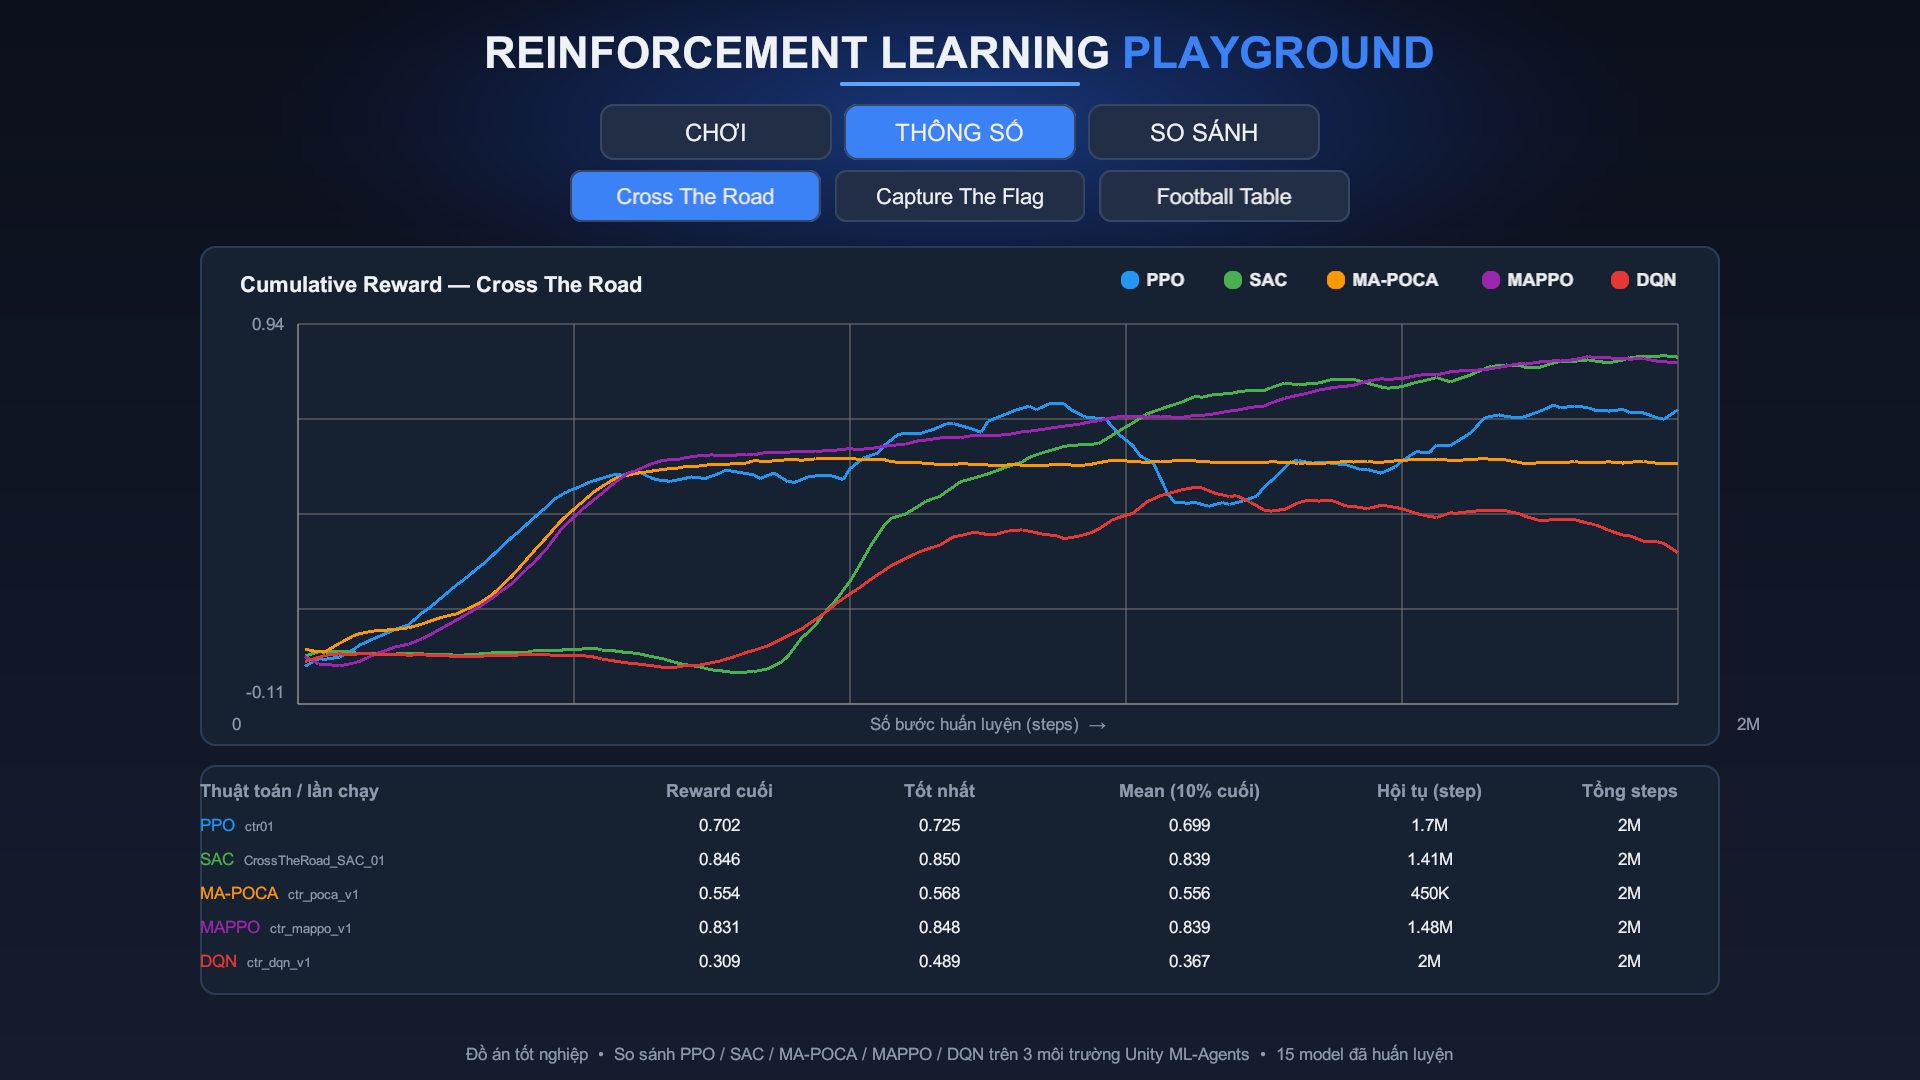
\includegraphics[width=0.97\textwidth]{image/app/app_menu_stats.png}
\caption{Tab THÔNG SỐ: đường cong phần thưởng tích lũy và bảng thống kê của
năm thuật toán trên môi trường Cross The Road}
\label{fig:app_stats}
\end{figure}

\indent Bảng thống kê bên dưới biểu đồ liệt kê theo từng thuật toán các cột: phần
thưởng cuối, phần thưởng tốt nhất, trung bình mười phần trăm cuối, bước hội tụ ước
lượng và tổng số bước. Cột đầu ghi tên thuật toán kèm mã lần chạy ở cỡ chữ nhỏ, để mỗi
dòng chỉ đích danh mô hình đã sinh ra con số đó. Những thuật toán chưa được huấn luyện
trên môi trường đó hiển thị ``N/A'' thay vì bị ẩn đi, nhờ vậy người xem thấy rõ phạm vi
thực nghiệm của đề tài đến đâu. Đại lượng được vẽ ở đây là phần thưởng tích lũy môi trường
(\texttt{Environment/Cumulative Reward}) lấy nguyên từ nhật ký huấn luyện, nên thang
giá trị có thể lệch so với các đường cong phần thưởng ngoại sinh ở
Chương~\ref{ch:results}. Hai tab số liệu trong ứng dụng phục vụ tra cứu nhanh, không
thay thế phần phân tích chi tiết của báo cáo.

\subsubsection{Tab SO SÁNH}

\indent Tab \textit{SO SÁNH} (Hình~\ref{fig:app_compare}) đưa ba môi trường lên cùng
một màn hình. Mỗi môi trường là một thẻ chứa biểu đồ cột, mỗi cột là một thuật toán
với chiều cao tỉ lệ theo phần thưởng trung bình mười phần trăm cuối và được tô đúng
màu quy ước; giá trị số được ghi ngay trên đỉnh cột. Do thang phần thưởng của ba môi
trường rất khác nhau (Football Table dùng thang lớn hơn hẳn hai môi trường còn lại),
chiều cao cột được chuẩn hóa theo giá trị lớn nhất trong từng thẻ chứ không
dùng chung một trục; nhờ vậy việc so sánh luôn diễn ra trong nội bộ một môi trường,
đúng với kết luận xuyên suốt của đề tài rằng thứ hạng thuật toán chỉ có ý nghĩa khi
gắn với một dạng bài toán cụ thể. Bảng xếp hạng phía dưới liệt kê đủ cả năm vị trí của
từng môi trường chứ không cắt ở ba vị trí đầu, cho phép đọc ngay kết luận so sánh - kể
cả thuật toán xếp cuối - mà không cần nhìn biểu đồ.
Có một chỗ vênh cần nói rõ: bảng xếp hạng trong ứng dụng sắp thứ tự thuần theo phần
thưởng, nên với Football Table nó không trùng với thứ hạng ở
Bảng~\ref{tab:overall_ranking}, nơi môi trường đối kháng được xếp theo mức tăng chỉ số
ELO như đã lập luận ở Mục~\ref{ch:results}.

\begin{figure}[H]
\centering
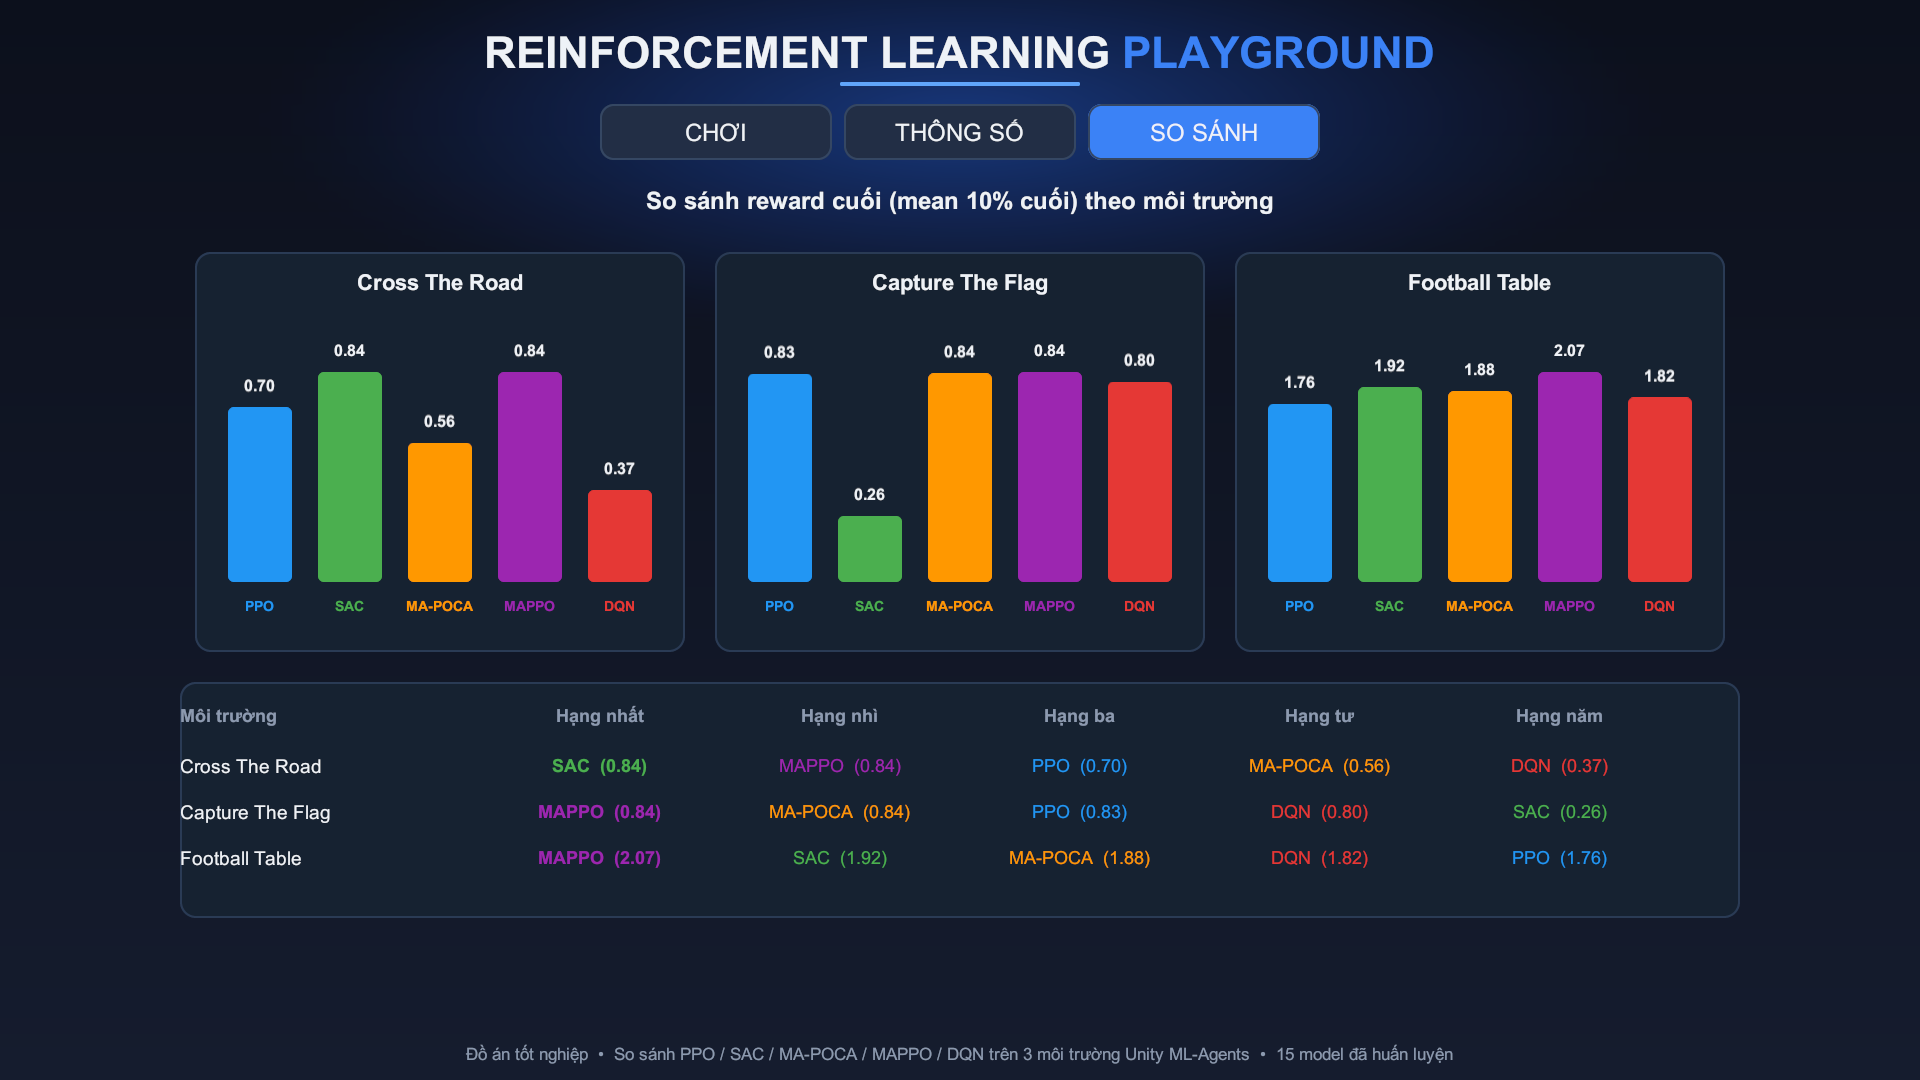
\includegraphics[width=0.97\textwidth]{image/app/app_menu_compare.png}
\caption{Tab SO SÁNH: biểu đồ cột theo từng môi trường và bảng xếp hạng
thuật toán}
\label{fig:app_compare}
\end{figure}

% ───────────────────────────────────────────────
\subsection{Ba chế độ chơi trong từng môi trường}
\label{sub:app-modes}

\indent Do bản chất khác nhau (đơn tác nhân, hợp tác, đối kháng), ba chế độ chơi được
ánh xạ vào mỗi môi trường theo một cách riêng, tổng hợp trong
Bảng~\ref{tab:app_mode_matrix}.

\begin{table}[H]
\centering
\caption{Ánh xạ ba chế độ chơi vào ba môi trường}
\label{tab:app_mode_matrix}
\renewcommand{\arraystretch}{1.35}
\tablefont
\begin{tabular}{|>{\raggedright\arraybackslash}p{2.4cm}
                |>{\raggedright\arraybackslash}p{3.6cm}
                |>{\raggedright\arraybackslash}p{3.6cm}
                |>{\raggedright\arraybackslash}p{3.6cm}|}
\hline
\textbf{Môi trường} & \textbf{Người chơi} & \textbf{Agent tự chơi} & \textbf{Chơi với Agent} \\
\hline
Cross The Road & Người điều khiển nhân vật trong khu vực & Mô hình điều khiển nhân vật trong khu vực & Người và tác nhân đua song song ở hai khu vực liền kề \\
\hline
Capture The Flag & Hai người chơi trên cùng bàn phím & Hai tác nhân cùng dùng một mô hình & Người phối hợp cùng tác nhân đồng đội \\
\hline
Football Table & Người đấu với bot luật đơn giản & Mô hình đấu với mô hình (cùng loại hành động)$^{*}$ & Người đấu với mô hình \\
\hline
\multicolumn{4}{|p{14.2cm}|}{$^{*}$ Hai ô mô hình phải cùng dùng hành động liên tục
hoặc cùng rời rạc, vì mỗi loại chạy trên một bản scene riêng; xem
Mục~\ref{sub:app-model}.} \\
\hline
\end{tabular}
\end{table}

\subsubsection{Cross The Road: trải nghiệm và quan sát chính sách}

\indent Ở chế độ \textit{Người chơi}, người dùng điều khiển nhân vật bằng các phím mũi
tên (hoặc A/D/W) đúng theo bốn hành động rời rạc mà tác nhân được phép dùng khi huấn
luyện: đứng yên, sang trái, sang phải và tiến lên. Việc ràng buộc người chơi vào đúng
không gian hành động của tác nhân là có chủ đích: ràng buộc này giúp người dùng đánh giá đúng độ khó của bài toán, thay vì được điều
khiển tự do hơn tác nhân và đi tới kết luận sai lệch.

\indent Ở chế độ \textit{Agent tự chơi}, mọi tác nhân trong scene được chuyển sang
suy luận bằng mô hình đã chọn và camera tự động đóng khung vào vùng chơi
(Hình~\ref{fig:app_ctr_agent}). Thanh thông tin phía trên hiển thị tên mô hình đang
chạy, còn bảng chỉ số dựng sẵn trong môi trường hiển thị phần thưởng tích lũy, số tập
đã hoàn thành và số bước của tập hiện tại; nhờ vậy người xem đối chiếu được ngay giữa
hành vi quan sát được và chỉ số mà mô hình đạt được. Đây cũng là cách trực quan nhất
để thấy khác biệt giữa các thuật toán: mô hình SAC băng qua đường với ít va chạm hơn,
trong khi mô hình MAPPO thường dừng lại lâu hơn ở các làn có mật độ phương tiện cao,
phù hợp với thứ hạng phần thưởng đã trình bày ở Chương~\ref{ch:results}.

\begin{figure}[H]
\centering
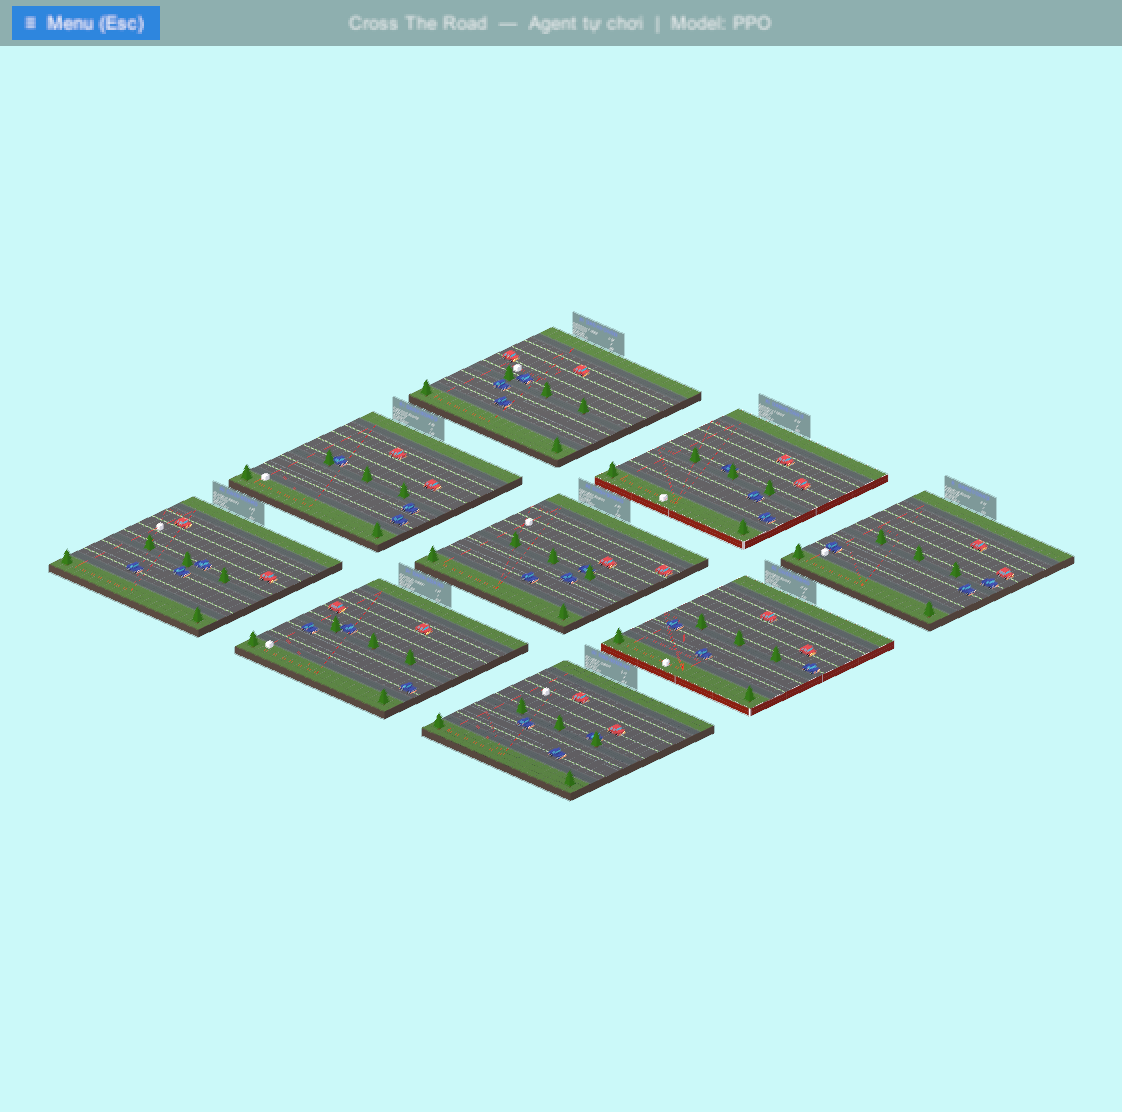
\includegraphics[width=0.78\textwidth]{image/app/app_ctr_agent.png}
\caption{Chế độ Agent tự chơi trong Cross The Road: mô hình
\texttt{ctr\_mappo\_v1} điều khiển tác nhân, chỉ số hiển thị trực tiếp trong cảnh}
\label{fig:app_ctr_agent}
\end{figure}

\indent Chế độ còn lại của môi trường này (\textit{Chơi với Agent}) được thiết kế theo
mô hình đua song song: ứng dụng giữ lại hai khu vực huấn luyện cạnh nhau, tắt các khu
vực còn lại, giao khu vực bên trái cho người chơi và khu vực bên phải cho tác nhân
máy, rồi tính lại khung nhìn để cả hai khu vực cùng nằm gọn trong màn hình. Scene
Cross The Road hiện chứa tám khu vực huấn luyện nên chế độ này dùng được; số khu vực
dư ra không gây ảnh hưởng vì chúng bị tắt ngay khi scene nạp xong.

\subsubsection{Capture The Flag: phối hợp người - máy}

\indent Môi trường hợp tác cho phép một kịch bản đáng chú ý: con người phối hợp
với tác nhân máy trong cùng một đội. Ở chế độ \textit{Chơi với Agent}, người chơi
điều khiển một nhân vật bằng các phím W A S D (kèm Q/E để đi ngang), còn nhân vật thứ
hai do mô hình đã chọn điều khiển (Hình~\ref{fig:app_ctf_pva}). Nhiệm vụ đòi hỏi đúng
chuỗi phối hợp đã phân tích ở Mục~\ref{sub:env-coop}: một bên đứng lên bàn đạp giữ
cửa, bên kia đi qua, rồi đổi vai - người chơi vì vậy phải suy đoán được ý định của
đồng đội máy và hành động ăn khớp, qua đó minh họa trực tiếp cho khái niệm phối hợp
đa tác nhân.

\begin{figure}[H]
\centering
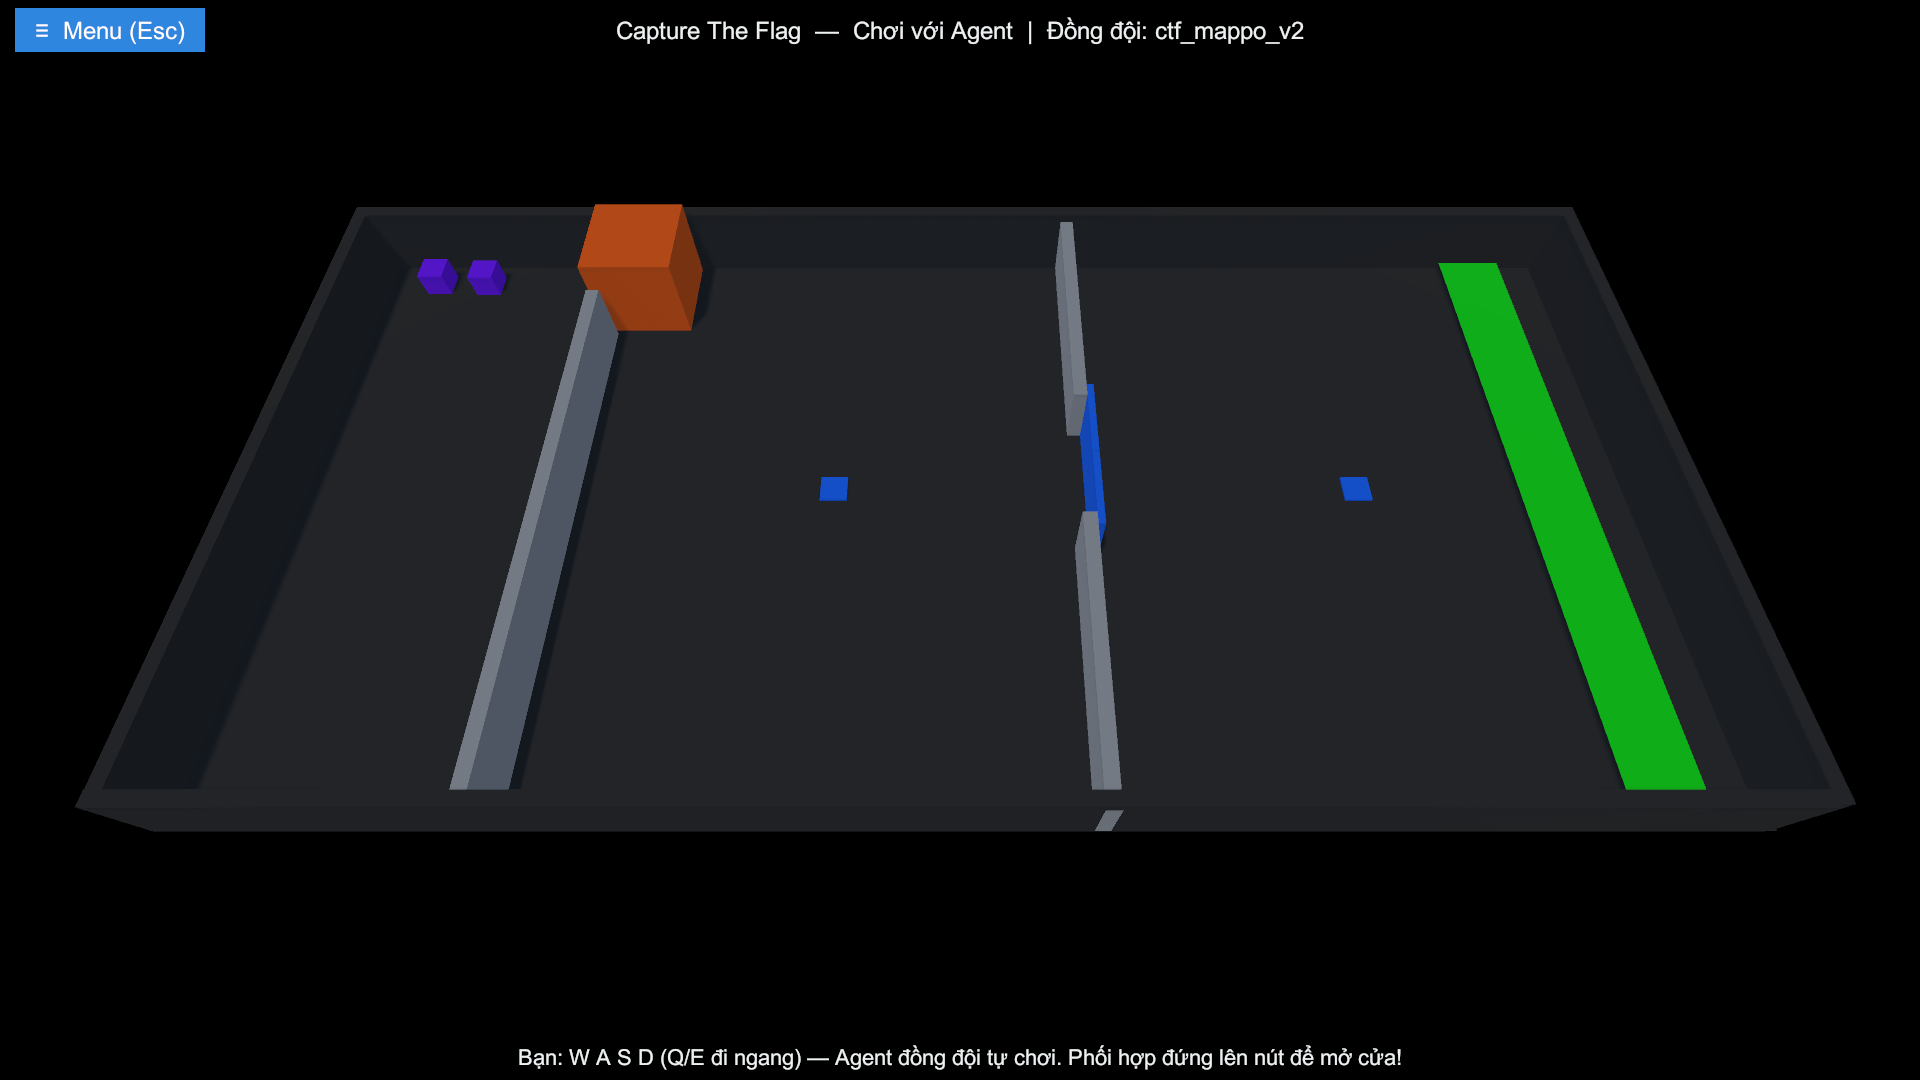
\includegraphics[width=0.78\textwidth]{image/app/app_ctf_pva.png}
\caption{Chế độ Chơi với Agent trong Capture The Flag: người chơi phối hợp
cùng tác nhân đồng đội dùng mô hình \texttt{ctf\_mappo\_v2}}
\label{fig:app_ctf_pva}
\end{figure}

\indent Ở chế độ \textit{Người chơi}, cả hai nhân vật đều do con người điều khiển
theo kiểu hai người chơi chung bàn phím: một người dùng cụm W A S D (Q/E đi
ngang), người còn lại dùng cụm phím mũi tên (dấu ngoặc vuông để đi ngang). Chế độ
\textit{Agent tự chơi} để cả hai nhân vật chạy cùng một mô hình, tái hiện đúng cấu
hình lúc huấn luyện vì hai tác nhân vốn chia sẻ chung một chính sách.

\subsubsection{Football Table: đối đầu người - máy và máy - máy}

\indent Trong môi trường đối kháng, chế độ \textit{Chơi với Agent} cho người chơi
cầm đội Xanh đấu trực tiếp với mô hình ở đội Đỏ. Vì mỗi đội có bốn thanh gạt với tám
kênh điều khiển liên tục, sơ đồ phím được thiết kế theo nguyên tắc ``một thanh tại
một thời điểm'': phím Q/E hoặc các phím số 1-4 chọn thanh đang điều khiển, W/S trượt
thanh và A/D xoay thanh để sút (Hình~\ref{fig:app_fb_player}); tên thanh đang chọn
(thủ môn, hậu vệ, tiền vệ, tiền đạo) hiển thị ở góc trên trái màn hình. Giá trị hành
động do người chơi sinh ra còn được nhân với dấu của đội, đúng như cách chuẩn hóa hệ
tọa độ khi huấn luyện, nhờ vậy cùng một sơ đồ phím dùng được cho cả hai phía sân. Ở
chế độ \textit{Người chơi}, đối thủ là bot luật cố định bám theo vị trí bóng - chính
là đối thủ mốc đã dùng khi huấn luyện ở Mục~\ref{sub:env-football} - với độ khó vừa
phải, phù hợp để người dùng làm quen với sơ đồ điều khiển trước khi đối đầu với các
mô hình đã huấn luyện.

\begin{figure}[H]
\centering
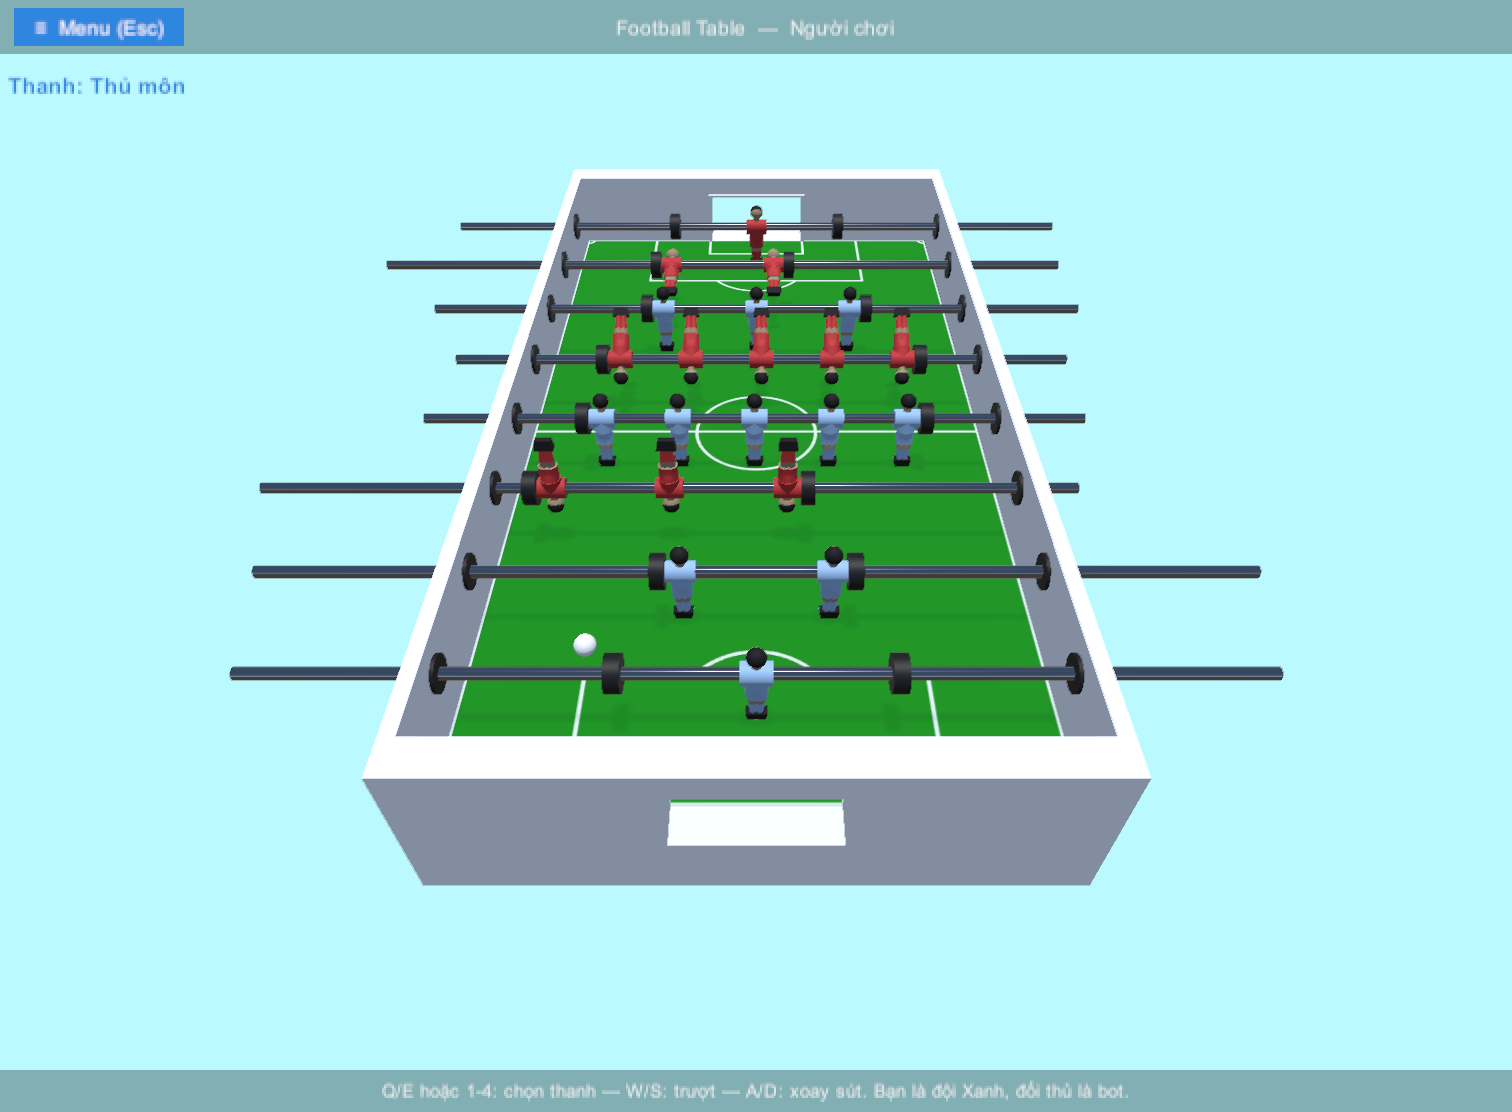
\includegraphics[width=0.78\textwidth]{image/app/app_fb_player.png}
\caption{Chế độ Người chơi trong Football Table: người chơi cầm đội Xanh,
góc trên trái hiển thị thanh gạt đang được chọn}
\label{fig:app_fb_player}
\end{figure}

\indent Đáng chú ý nhất là chế độ \textit{Agent tự chơi} với hai ô chọn mô hình độc
lập: người dùng có thể cho mô hình PPO huấn luyện bằng tự chơi đấu với mô hình
MA-POCA, MAPPO hoặc SAC, hoặc cho hai bản sao của cùng một mô hình đối đầu; thanh thông
tin phía trên hiển thị đồng thời tên mô hình của cả hai đội. Riêng mô hình DQN chỉ đấu
được với chính nó vì nó là chính sách rời rạc duy nhất trên môi trường này, và trận đấu
đó chạy trên bản scene rời rạc (Hình~\ref{fig:app_fb_dqn}). Đây thực chất là một công cụ
đánh giá đối kháng trực tiếp thu nhỏ, bổ sung một kênh so sánh định
tính cho các kết quả định lượng ở Chương~\ref{ch:results}: hai mô hình có phần thưởng
trung bình gần nhau vẫn có thể cho ra thế trận rất khác nhau khi gặp trực tiếp.

\begin{figure}[H]
\centering
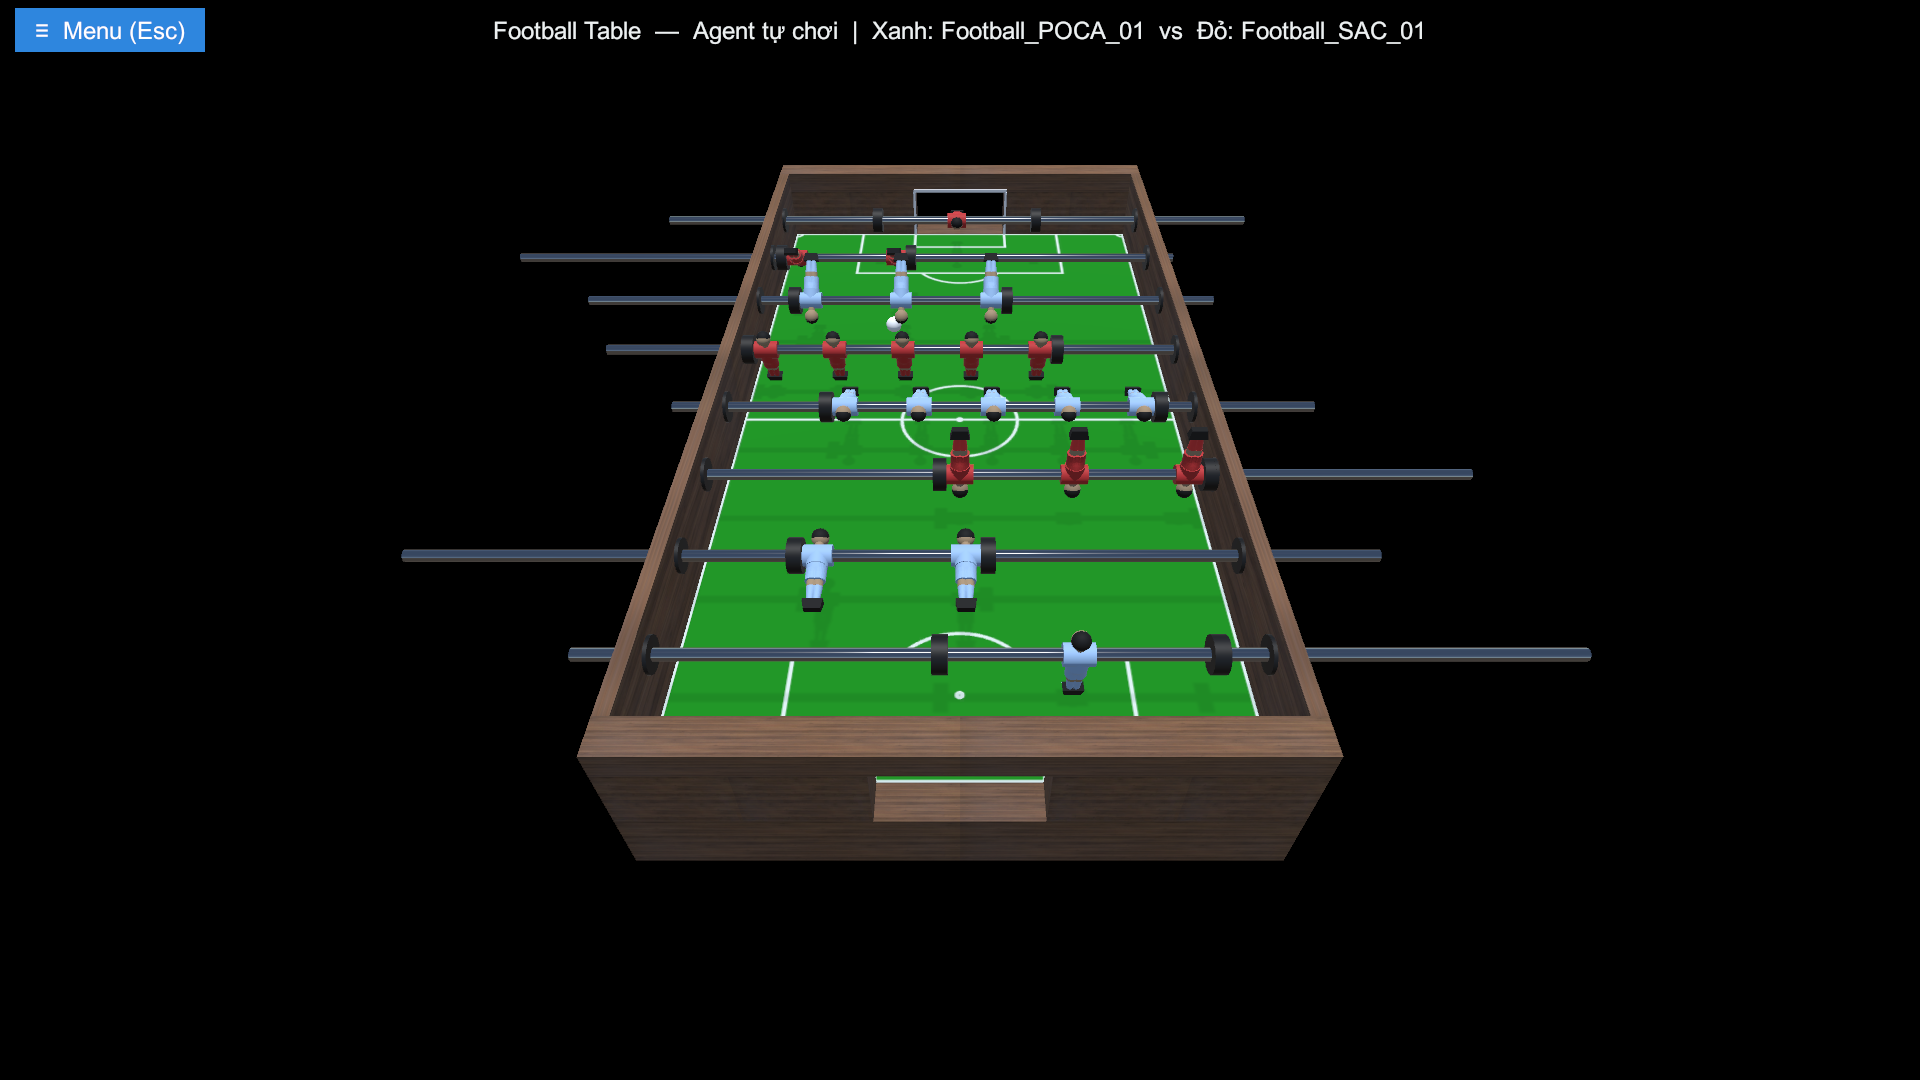
\includegraphics[width=0.78\textwidth]{image/app/app_fb_agent.png}
\caption{Chế độ Agent tự chơi trong Football Table với mô hình
\texttt{football\_dqn\_v1}: ứng dụng nạp bản scene rời rạc và chỉ giữ lại một bàn
trong số tám bàn của cấu hình huấn luyện}
\label{fig:app_fb_dqn}
\end{figure}

% ───────────────────────────────────────────────
\subsection{Đóng gói ba môi trường thành gói dùng lại được}
\label{sub:app-package}

\indent Ba môi trường của đề tài được xây dựng cho một mục đích cụ thể là so sánh
thuật toán, nhưng bản thân chúng có giá trị dùng lại: một lập trình viên Unity muốn
thử nghiệm học tăng cường thường mất phần lớn thời gian ở khâu dựng môi trường chứ
không phải ở khâu chọn thuật toán. Vì vậy đề tài đóng gói cả ba môi trường thành một
gói UPM (\textit{Unity Package Manager}) tên \texttt{com.vanhuyen.rl-game-envs}, cài
được vào một dự án Unity bất kỳ như mọi gói chính thức khác.

\subsubsection{Cấu trúc gói}

\indent Gói tuân theo bố cục chuẩn của UPM, tóm tắt trong
Bảng~\ref{tab:pkg_layout}. Điểm đáng nói không nằm ở danh sách thư mục mà ở ranh giới
giữa chúng: toàn bộ mã điều khiển môi trường nằm trong \texttt{Runtime} và được biên
dịch thành một assembly riêng, tách khỏi \texttt{Assembly-CSharp} của dự án. Nhờ đó
trình biên dịch tự canh giữ tính độc lập của gói - nếu một lớp môi trường lỡ tham
chiếu tới mã của ứng dụng trình diễn thì dự án không biên dịch được nữa, chứ không
phải chờ tới lúc người khác cài gói mới phát hiện ra.

\begin{table}[H]
\centering
\caption{Bố cục gói \texttt{com.vanhuyen.rl-game-envs}}
\label{tab:pkg_layout}
\renewcommand{\arraystretch}{1.3}
\tablefont
\begin{tabular}{|p{3.6cm}|>{\raggedright\arraybackslash}p{9.9cm}|}
\hline
\textbf{Thư mục} & \textbf{Nội dung} \\
\hline
\texttt{Runtime/} & 36 lớp điều khiển của ba môi trường (tác nhân, quan sát, hàm
phần thưởng, sinh vật cản, trọng tài) cùng giao diện
\texttt{IManualActionSource}; một assembly riêng. \\
\hline
\texttt{Editor/} & Trình hướng dẫn cài đặt và bốn công cụ: nhân khu vực huấn luyện,
build headless, sinh bản scene hành động rời rạc, cài cấu hình huấn luyện. \\
\hline
\texttt{Configs/} & Mười lăm tệp YAML cho năm thuật toán trên ba môi trường. \\
\hline
\texttt{Samples\textasciitilde/} & Bốn mẫu import được từ Package Manager: ba môi
trường (scene, prefab, vật liệu, thiết lập vật lý) và bộ cấu hình huấn luyện. \\
\hline
\texttt{Documentation\textasciitilde/} & Tài liệu hướng dẫn, kèm \texttt{README},
\texttt{CHANGELOG} và \texttt{LICENSE} ở gốc gói. \\
\hline
\end{tabular}
\end{table}

\subsubsection{Gỡ phụ thuộc ngược từ môi trường vào ứng dụng}

\indent Muốn đóng gói được thì trước hết phải gỡ một phụ thuộc sai chiều đã tồn tại
sẵn. Hàm \texttt{Heuristic} của cả ba tác nhân trước đây gọi thẳng
\texttt{GetComponent} tới các lớp cụ thể của ứng dụng trình diễn để lấy hành động do
người chơi nhập vào. Quan hệ này ngược với thứ bậc đúng: môi trường là tầng dưới,
đáng lẽ không được biết gì về ứng dụng nhúng nó. Trong một dự án đơn lẻ thì điều đó vô
hại, nhưng khi tách gói ra thì nó thành lỗi biên dịch thực sự, vì một gói không được
phép tham chiếu tới assembly mặc định của dự án.

\indent Đề tài đảo chiều phụ thuộc bằng một giao diện đặt trong chính gói:

\begin{lstlisting}[language={[Sharp]C}, caption={Giao diện cho nguồn điều khiển thủ công}]
public interface IManualActionSource
{
    void WriteActions(in ActionBuffers actionsOut);
}
\end{lstlisting}

\indent Hàm \texttt{Heuristic} của môi trường nay chỉ hỏi ``có thành phần nào trên
GameObject này hiện thực giao diện đó không''; có thì giao quyền quyết định, không thì
quay về sơ đồ phím mặc định. Ứng dụng trình diễn trở thành một bên hiện thực giao diện
như mọi bên khác, và người dùng gói muốn thêm một cách điều khiển mới - gamepad, kịch
bản kiểm thử tự động, hay chính mô hình ngôn ngữ lớn - chỉ cần viết một
\texttt{MonoBehaviour} rồi gắn vào, không phải sửa một dòng nào trong mã môi trường.

\indent Một chi tiết phải xử lý kèm là hai không gian hành động của Football Table đã
nói ở Mục~\ref{sub:app-model}. Nếu để mỗi nguồn điều khiển tự lo việc ghi ra hành động
liên tục hay rời rạc thì đoạn quy đổi ba mức sẽ bị chép lại ở mọi nơi. Gói vì thế cung
cấp sẵn một hàm tiện ích: nguồn điều khiển chỉ sinh ra ý định trong đoạn $[-1,1]$, còn
việc brain nào đang chạy là chuyện của gói.

\subsubsection{Trình hướng dẫn cài đặt}

\indent Rào cản lớn nhất với người mới không phải là thiếu tài liệu mà là không biết
mình đang đứng ở đâu trong tài liệu đó. Đề tài vì vậy viết một cửa sổ Editor
(Hình~\ref{fig:pkg_wizard}) chia toàn bộ quy trình thành bảy bước, và điểm mấu chốt là
mỗi bước \textit{tự kiểm tra trạng thái hiện tại} rồi hiển thị dấu tích hoặc nút hành
động tương ứng, thay vì chỉ liệt kê việc cần làm.

\begin{figure}[H]
\centering
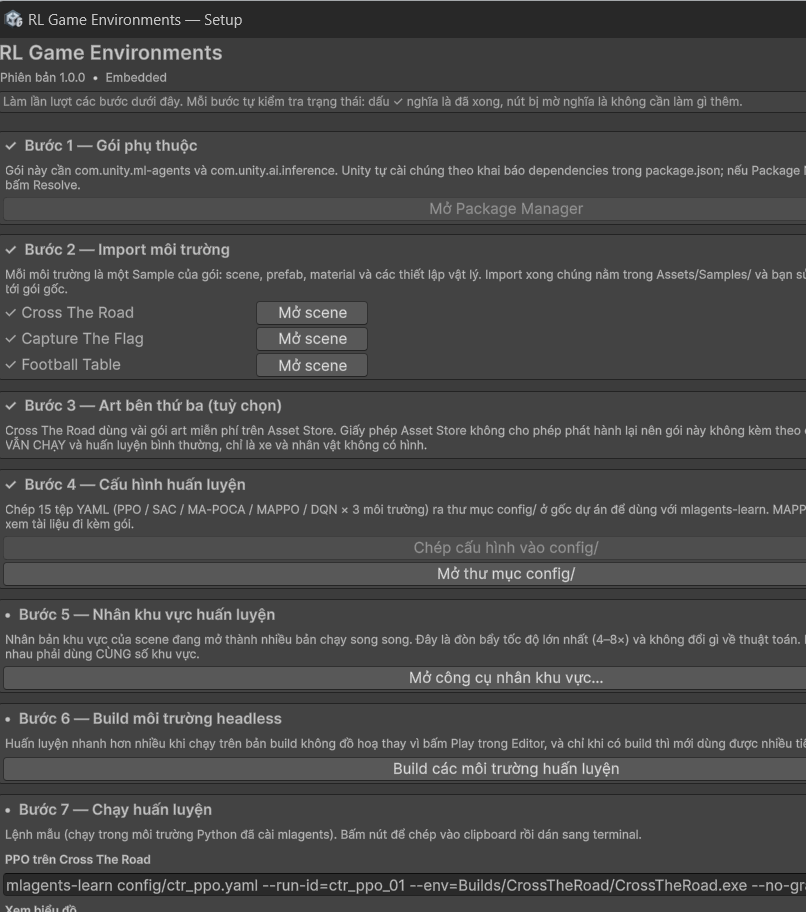
\includegraphics[width=0.82\textwidth]{image/app/app_pkg_wizard.png}
\caption{Trình hướng dẫn cài đặt của gói: bảy bước, mỗi bước tự kiểm tra trạng thái
và chỉ bật nút khi thực sự còn thiếu}
\label{fig:pkg_wizard}
\end{figure}

\indent Bảy bước lần lượt là: kiểm tra gói phụ thuộc; import môi trường từ mục Samples
của Package Manager; kiểm tra các gói art bên thứ ba; chép cấu hình huấn luyện ra thư
mục \texttt{config/}; nhân khu vực huấn luyện; build môi trường headless; và cuối cùng
là lệnh mẫu để chạy huấn luyện, kèm nút chép sang clipboard. Ba bước giữa gọi lại đúng
những công cụ mà đề tài đã dùng cho phần thực nghiệm của mình, nên người dùng gói đi
theo cùng một quy trình đã được kiểm chứng chứ không phải quy trình viết riêng cho tài
liệu.

\indent Bước kiểm tra art bên thứ ba tồn tại vì một ràng buộc pháp lý. Môi trường Cross
The Road hiển thị bằng vài gói art miễn phí trên Unity Asset Store; giấy phép Asset
Store cho phép dùng trong dự án của người đã tải nhưng không cho phép đóng gói lại để
phát hành cho người khác, kể cả khi gói art đó miễn phí. Gói của đề tài vì thế không
kèm chúng. Đây là một hạn chế thật chứ không phải chi tiết thủ tục, nên trình hướng dẫn
xử lý nó một cách rõ ràng: quét dự án xem thiếu gói nào, nêu đích danh, mở thẳng trang
tải, và nói rõ rằng thiếu art thì môi trường vẫn huấn luyện bình thường - chỉ là xe và
nhân vật không có hình. Phần mã nguồn và cấu hình do đề tài viết được phát hành theo
giấy phép MIT.

\subsubsection{Dự án tự dùng chính gói của mình}

\indent Gói được đặt ở dạng nhúng ngay trong thư mục \texttt{Packages/} của dự án, và
ứng dụng trình diễn ở các mục trước tiêu thụ nó đúng theo cách một dự án bên ngoài sẽ
làm: qua ranh giới assembly, qua giao diện công khai, không có đường tắt nào. Cách bố
trí này biến toàn bộ phần thực nghiệm và phần trình diễn của đồ án thành một phép kiểm
thử thường trực cho gói - mỗi lần chạy lại các luồng ở
Bảng~\ref{tab:app_test} cũng là một lần xác nhận gói còn dùng được, thay vì phải tin
vào một bản đóng gói chỉ được thử đúng một lần lúc phát hành.

% ───────────────────────────────────────────────
\subsection{Các vấn đề kỹ thuật và giải pháp}
\label{sub:app-issues}

\indent Quá trình xây dựng ứng dụng phát sinh một số vấn đề kỹ thuật đặc thù của việc
ghép nối vòng lặp quyết định của ML-Agents với tương tác thời gian thực của người
chơi; các vấn đề tiêu biểu và giải pháp tương ứng được tổng hợp dưới đây.

\indent \textbf{Độ trễ điều khiển do chu kỳ quyết định:} Khi huấn luyện, các tác nhân
chỉ yêu cầu quyết định sau mỗi vài bước vật lý (thành phần
\texttt{DecisionRequester}) nhằm giảm chi phí tính toán. Tần suất này khiến nhân vật
phản hồi phím rất chậm ở chế độ người chơi. Giải pháp là khi cấu hình tác nhân cho
người điều khiển, chu kỳ quyết định được hạ xuống 1 - tác nhân yêu cầu
quyết định ở mọi bước vật lý - trong khi các tác nhân máy giữ nguyên chu kỳ gốc để tái
hiện đúng điều kiện huấn luyện.

\indent \textbf{Mất phím bấm giữa hai lần quyết định:} Hàm \texttt{Heuristic} của
Cross The Road đọc sự kiện nhấn phím tức thời; nếu người chơi nhấn phím vào một khung
hình không trùng thời điểm lấy quyết định thì thao tác bị bỏ sót. Đề tài bổ sung một
thành phần đệm đầu vào: phím được ghi nhận trong vòng lặp \texttt{Update} (chạy mỗi
khung hình) và giữ lại cho đến khi hàm \texttt{Heuristic} tiêu thụ ở lần quyết định
kế tiếp, bảo đảm không thao tác nào bị mất.

\indent \textbf{Đóng khung camera với máy quay trực giao:} Scene Cross The Road dùng
một máy quay trực giao bao quát toàn bộ khu vực huấn luyện; khi số khu vực còn hoạt
động thay đổi theo chế độ chơi, khung hình gốc không còn phù hợp. Ứng dụng tính
hộp bao của các khu vực còn hoạt động, dời máy quay về trục nhìn đi qua tâm hộp và
đặt lại kích thước trực giao bằng cách chiếu tám đỉnh hộp lên hai trục ngang - dọc
của máy quay. Phép đóng khung này được hoãn đến cuối khung hình đầu tiên, vì tại thời
điểm scene vừa nạp xong, các phương tiện chưa được đặt về đúng vị trí xuất phát nên
hộp bao tính sớm sẽ bị sai lệch.

\indent \textbf{Xung đột thứ tự khởi tạo trong Football Table:} Thành phần
\texttt{Agent} của ML-Agents có thể gọi \texttt{OnEpisodeBegin}, kéo theo việc đặt
lại bàn và bóng, ngay trong pha \texttt{OnEnable} và do đó chạy trước khi bộ khởi tạo
của scene kịp hoàn tất, gây lỗi tham chiếu rỗng ngắt quãng. Đề tài sửa các lớp
\texttt{Team} và \texttt{Ball} theo hướng tự khởi tạo an toàn: thao tác đặt lại sẽ tự
gọi khởi tạo nếu phát hiện chưa được khởi tạo, còn việc khởi tạo lặp được chặn bằng
cờ trạng thái.

\indent \textbf{Tác nhân thừa ở chế độ người chơi:} Trong Football Table chế độ
\textit{Người chơi}, đội Đỏ do bot luật điều khiển trực tiếp, nhưng tác nhân
ML-Agents của đội này vẫn tồn tại trong scene và có thể phát sinh hành động nhiễu.
Giải pháp là vô hiệu hóa bộ yêu cầu quyết định của tác nhân đó (để nó không bao giờ
yêu cầu quyết định mới) và đặt giới hạn bước của tập về không, nhờ vậy các sự kiện
bàn thắng và việc đặt lại trận đấu vẫn được xử lý bình thường.

\indent \textbf{Nhiều khu vực huấn luyện trong một scene:} Để tăng tốc thu thập kinh
nghiệm, ba scene môi trường đã được nhân bản khu vực huấn luyện lên tám bản chạy song
song, các bản sao nằm gọn trong một đối tượng chứa chung. Ứng dụng ban đầu được viết
cho scene một khu vực nên xác định khu vực bằng đối tượng gốc của tác nhân; sau khi
nhân bản, mọi bản sao có chung một đối tượng gốc và cách xác định này sụp đổ. Hậu quả
nặng nhất rơi vào Football Table: quy tắc ``đội Đỏ là tác nhân đầu tiên không phải đội
Xanh'' chọn trúng một tác nhân Xanh của bàn khác, nên trận đấu không bao giờ hình
thành và mười bốn tác nhân còn lại vẫn chạy ở cấu hình huấn luyện. Đề tài sửa bằng
cách xác định khu vực theo cấu trúc cây: đi ngược lên cha cho tới ngay dưới đối tượng
chứa chung, nhờ đó cả bản gốc lẫn bản sao đều trả về đúng khu vực của mình. Trên nền
đó, các chế độ chơi giữ lại đúng số khu vực cần thiết (một bàn cho Football Table và
Capture The Flag, hai khu vực cho chế độ đua song song của Cross The Road) và tắt phần
còn lại, rồi chọn tác nhân trong phạm vi khu vực đã giữ.

\indent \textbf{Đóng khung camera cho vùng chơi dài và dẹt:} Việc chỉ giữ lại một khu
vực khiến khung nhìn gốc của scene không còn phù hợp, nhưng cách đóng khung ban đầu -
đặt camera cách tâm một khoảng tỉ lệ với bán kính hình cầu bao vùng chơi - lại đẩy
camera ra quá xa với những vùng chơi dài và dẹt như bàn bi lắc, khiến bàn chỉ chiếm
một phần nhỏ màn hình. Đề tài thay bằng phép chiếu tám đỉnh hộp bao lên ba trục của
camera: với máy quay trực giao thì tính kích thước trực giao vừa khít, còn với máy quay
phối cảnh thì tính khoảng cách nhỏ nhất để nửa chiều cao và nửa chiều rộng vẫn nằm
trong góc nhìn. Cách này dùng chung cho cả ba môi trường mà không cần tham số riêng.

\indent \textbf{Không gian hành động cố định từ lúc nạp scene:} Ứng dụng đổi được mô
hình của một tác nhân tại thời gian chạy, nhưng không đổi được \textit{kiểu} hành động
của nó: ML-Agents dựng bộ truyền động từ \texttt{BehaviorParameters} ngay trong pha
\texttt{OnEnable}, tức trước khi sự kiện nạp scene kịp báo về cho ứng dụng, và việc nạp
lại chính sách sau đó vẫn dùng đặc tả hành động đã dựng. Hệ quả là mô hình DQN rời rạc
của Football Table không thể chạy trên scene liên tục dù lớp tác nhân đã hỗ trợ cả hai
kiểu. Giải pháp là sinh sẵn một bản sao rời rạc của scene bằng kịch bản trong trình
soạn thảo và để menu chọn bản scene phù hợp với mô hình người dùng vừa chọn - đổi scene
thay vì đổi đặc tả hành động, nhờ đó không phải đụng tới scene gốc dùng cho huấn luyện.

\indent \textbf{Phạt thời gian chia cho không:} Chính việc đặt giới hạn bước về không
ở trên lại làm lộ một lỗi tiềm ẩn trong hàm phần thưởng của Football Table: thành phần
phạt thời gian được tính bằng nghịch đảo của giới hạn bước, nên khi giới hạn bằng
không, giá trị phần thưởng trở thành vô cực và ML-Agents ném ngoại lệ ở mỗi bước.
Đề tài sửa bằng cách chỉ áp dụng phạt thời gian khi giới hạn bước lớn hơn không, đúng
với ngữ nghĩa ``tập không giới hạn bước thì không có áp lực thời gian''. Đây là một ví
dụ điển hình cho việc chuyển một môi trường từ chế độ huấn luyện sang chế độ chơi có
thể kích hoạt những nhánh mã chưa từng được thực thi trong huấn luyện.

% ───────────────────────────────────────────────
\subsection{Kiểm thử ứng dụng và hạn chế}
\label{sub:app-testing}

\indent Ứng dụng được kiểm thử trực tiếp trong Unity Editor theo từng luồng chức
năng. Với mỗi tổ hợp môi trường - chế độ, quá trình kiểm thử xác nhận bốn điểm:
(1) scene được nạp và cấu hình đúng vai trò từng tác nhân (loại hành vi, mô hình,
chu kỳ quyết định); (2) mô hình ONNX được nạp thành công và tác nhân hành xử đúng
như kỳ vọng từ kết quả huấn luyện; (3) giao diện phủ hiển thị đúng thông tin và nút
quay về menu hoạt động; (4) không phát sinh lỗi nào trong bảng điều khiển của Unity.
Kết quả kiểm thử được tổng hợp trong Bảng~\ref{tab:app_test}.

\begin{table}[H]
\centering
\caption{Kết quả kiểm thử các luồng chức năng của ứng dụng}
\label{tab:app_test}
\renewcommand{\arraystretch}{1.3}
\tablefont
\begin{tabular}{|p{5.6cm}|p{5.6cm}|>{\centering\arraybackslash}p{2.4cm}|}
\hline
\textbf{Luồng kiểm thử} & \textbf{Nội dung xác nhận} & \textbf{Kết quả} \\
\hline
Menu: chọn môi trường, chế độ, mô hình & Giao diện cập nhật đúng; ô mô hình
hiện/ẩn theo ngữ cảnh & Đạt \\
\hline
Menu: xem trước 3D, tab THÔNG SỐ, SO SÁNH & Xoay/phóng to mượt; biểu đồ, chú giải và
bảng hiện đủ năm thuật toán, khớp \texttt{training\_data.json} & Đạt \\
\hline
Menu: duyệt danh mục mô hình & Mỗi môi trường liệt kê đủ 5 mô hình kèm tên thuật
toán và màu quy ước & Đạt \\
\hline
Cross The Road - Agent tự chơi & Cả tám khu vực cùng chạy mô hình đã chọn & Đạt \\
\hline
Cross The Road - Chơi với Agent & Giữ lại hai khu vực liền kề, tắt sáu khu vực còn
lại; người bên trái, mô hình bên phải & Đạt \\
\hline
Capture The Flag - Agent tự chơi & Giữ một khu vực, hai tác nhân cùng mô hình,
camera đóng khung đúng & Đạt \\
\hline
Football Table - Người chơi & Giữ một bàn; Xanh do người, Đỏ do bot luật điều
khiển & Đạt \\
\hline
Football Table - Agent tự chơi & Giữ một bàn; hai đội đúng hai mô hình đã chọn
& Đạt \\
\hline
Football Table - mô hình DQN & Nạp bản scene rời rạc; cảnh báo và khóa nút bắt đầu
khi ghép DQN với mô hình liên tục & Đạt \\
\hline
Quay về menu (nút và phím Esc) & Trở về menu, đổi lựa chọn, vào lại bình
thường & Đạt \\
\hline
Mở scene trực tiếp (không qua menu) & Cấu hình huấn luyện gốc được giữ
nguyên & Đạt \\
\hline
Gói môi trường: nhận diện và biên dịch & Package Manager nhận gói nhúng; assembly
riêng biên dịch được, ba scene không đứt tham chiếu script & Đạt \\
\hline
Gói môi trường: trình hướng dẫn & Bảy bước hiển thị đúng trạng thái đã/chưa xong;
các nút gọi đúng công cụ & Đạt \\
\hline
\end{tabular}
\end{table}

\indent Về hiệu năng, suy luận mạng nơ-ron cho các tác nhân đồng thời cùng với giao
diện không gây sụt giảm tốc độ khung hình đáng kể trên cấu hình thực nghiệm ở
Mục~\ref{sub:hardware}, khẳng định tính khả thi của việc nhúng trực tiếp các mô hình
đã huấn luyện vào sản phẩm game. Toàn bộ mười lăm mô hình ONNX đi kèm ứng dụng đều nạp
và vận hành chính xác với đúng phổ quan sát - hành động đã khai báo khi huấn luyện.

\indent Ứng dụng còn hai hạn chế đã biết. Thứ nhất, kích thước thư mục tài nguyên tăng
mạnh khi đóng gói đủ mười lăm mô hình: riêng năm mô hình của Capture The Flag đã chiếm
khoảng 325 MB, gấp nhiều lần tổng dung lượng của hai môi trường còn lại. Nguyên nhân
không nằm ở số lượng mô hình mà ở kiến trúc mạng: quan sát tín hiệu mục tiêu của môi
trường này khiến ML-Agents dựng bộ mã hóa theo kiểu siêu mạng (\textit{hypernetwork}),
trong đó một nhánh phụ sinh ra trọng số cho lớp ẩn chính, đẩy số tham số của một chính
sách nhỏ lên gần mười bảy triệu. Nếu cần giảm dung lượng bản phát hành thì phải huấn
luyện lại Capture The Flag với kiểu điều kiện hóa mục tiêu khác, chứ không phải bớt mô
hình đi. Thứ hai, hai tab số liệu phản ánh nội dung tệp
\texttt{training\_data.json} tại thời điểm xuất, nên sau mỗi đợt huấn luyện mới cần
chạy lại kịch bản xuất dữ liệu thì ứng dụng mới hiển thị số liệu cập nhật - đổi lại,
cùng lệnh đó cũng cập nhật luôn danh mục mô hình nên hai phần không thể lệch nhau.
